\documentclass[10pt,a4paper]{article}
\usepackage[T1]{fontenc}
\usepackage[utf8]{inputenc}
\usepackage[spanish,es-tabla]{babel}
\usepackage{lmodern}
\usepackage[margin=2cm,headheight=32pt]{geometry}
\usepackage{graphicx,booktabs,longtable,tabularx,array,amsmath}
\usepackage{xcolor,tikz}
\usetikzlibrary{positioning,arrows.meta,fit,backgrounds,babel}
\usepackage{enumitem}
\usepackage[section]{placeins}
\usepackage{float}
\usepackage{needspace}
\usepackage{fancyhdr}
\usepackage{microtype}
\usepackage{cite}
\usepackage[font=footnotesize,labelfont=bf,labelsep=period,tableposition=top]{caption}
\usepackage{parskip}
\PassOptionsToPackage{hyphens}{url}
\usepackage[hidelinks]{hyperref}
\hypersetup{pdftitle={Informe de Práctica I -- Evaluación comparativa del filtrado de dominios para control parental en PDNS, VPN y proxies},pdfauthor={Matías Vigneau Andrades},pdfsubject={Práctica I -- Universidad Diego Portales}}
\definecolor{udpblue}{HTML}{244A64}
\definecolor{softblue}{HTML}{EDF3F7}
\definecolor{softorange}{HTML}{FFF1DD}
\definecolor{softgreen}{HTML}{EBF5EE}
\pagestyle{fancy}
\fancyhf{}
\fancyhead[L]{
\includegraphics[width=1.2cm]{udp_logo.png}}
\fancyhead[R]{Facultad de Ingeniería y Ciencias}
\fancyfoot[R]{\thepage\hspace{0.02cm}}
\renewcommand{\headrulewidth}{0.9pt}
\renewcommand{\footrulewidth}{0.5pt}
\setlist{itemsep=3pt,topsep=5pt}
\setlength{\emergencystretch}{2em}
\renewcommand{\arraystretch}{1.15}
\newcolumntype{Y}{>{\raggedright\arraybackslash}X}

\begin{document}
\hypersetup{pageanchor=false}
\begin{titlepage}
\begin{center}
\vspace*{\baselineskip}
{\bfseries\fontsize{16}{19}\selectfont UNIVERSIDAD DIEGO PORTALES\\[0.5cm]}
{\fontsize{11}{13}\selectfont FACULTAD DE INGENIERÍA Y CIENCIAS\par}
\vspace*{0.5\baselineskip}
{\bfseries\fontsize{10}{12}\selectfont ESCUELA DE INFORMÁTICA Y TELECOMUNICACIONES\\[0.35cm]}
\vspace*{\baselineskip}

\includegraphics[scale=0.40]{udp_logo.png}\par
\vspace*{3\baselineskip}
\hrule height 0.5pt
\vspace{1mm}
\hrule height 1.5pt
\vspace*{\baselineskip}
{\bfseries\fontsize{14}{17}\selectfont Informe de Práctica I\\[0.5cm]}
{\bfseries\itshape\fontsize{12}{15}\selectfont Evaluación comparativa del filtrado de dominios para control parental\\en servicios de Protective DNS (PDNS), VPN y proxies\par}
\vspace*{\baselineskip}
\hrule height 0.5pt
\vspace{1mm}
\hrule height 1.5pt
\vspace*{4.5\baselineskip}
{\bfseries\fontsize{14}{17}\selectfont Profesor Guía: }{\fontsize{12}{15}\selectfont Nicolás Boettcher}\\[0.3cm]
{\bfseries\fontsize{14}{17}\selectfont Alumno: }{\fontsize{12}{15}\selectfont Matías Vigneau Andrades}\\[0.3cm]
\vspace{0.8cm}
{\fontsize{10}{12}\selectfont 26 de noviembre de 2026\par}
\end{center}
\end{titlepage}

\tableofcontents
\thispagestyle{empty}
\clearpage
\setcounter{page}{1}
\hypersetup{pageanchor=true}

\section{Antecedentes y Motivación}

El Sistema de Nombres de Dominio (DNS) traduce nombres legibles para las personas en información de direccionamiento de red, como direcciones IPv4 mediante registros \texttt{A} \cite{rfc1034,rfc1035} y direcciones IPv6 mediante registros \texttt{AAAA} \cite{rfc3596}. En su operación ordinaria, un resolutor recursivo consulta servidores autoritativos o reutiliza registros guardados temporalmente en caché sin evaluar el tipo de contenido que aloja el sitio, utilizando tanto transporte clásico por puerto 53 (UDP y TCP \cite{rfc7766}) como canales cifrados mediante DNS sobre HTTPS (\emph{DNS over HTTPS}, DoH \cite{rfc8484}) y DNS sobre TLS (\emph{DNS over TLS}, DoT \cite{rfc7858}). Sobre esta infraestructura surgieron los servicios de \emph{Protective DNS} (PDNS), denominación estándar en la literatura para los resolutores que aplican reglas de filtrado y técnicas de reescritura de respuestas DNS (\emph{DNS rewriting}) con el fin de bloquear o redirigir dominios asociados a riesgos de seguridad o categorías restringidas \cite{liu2024,plonka2025}.

En la operación real, esta protección no se aplica de manera uniforme, ya que un mismo operador de PDNS suele ofrecer varios \emph{perfiles}, entendidos como configuraciones diferenciadas con una dirección o punto de acceso específico y una política de filtrado declarada por el proveedor. Cloudflare, por ejemplo, ofrece variantes separadas para resolución ordinaria, bloqueo de amenazas y protección familiar con contenido adulto, mientras Quad9 mantiene una variante de seguridad contra amenazas y otra sin bloqueo \cite{cloudflare,quad9}. Como documentan Liu et al. \cite{liu2024}, los proveedores modifican las respuestas bloqueadas de maneras distintas (direcciones especiales, páginas de aviso, respuestas negativas o códigos de error extendido DNS \cite{rfc8914}), por lo que conocer solo el nombre comercial de un servicio no basta para interpretar qué ocurre frente a cada consulta.

Ahora bien, el filtrado de dominios en red no depende únicamente de configurar manualmente un perfil PDNS, pues las redes privadas virtuales (VPN) y los proxies HTTP o SOCKS5 también interceptan o redirigen las consultas \cite{rfc9110,rfc1928}. A diferencia de la denominación \emph{Protective DNS} (PDNS), las especificaciones técnicas y los estudios sobre intermediarios consultados en este trabajo \cite{rfc9110,rfc1928,khan2018vpn,tsirantonakis2018proxy} no adoptan siglas equivalentes (como «PVPN» o «PProxy») para designar VPN o proxies con filtrado DNS; además, estos intermediarios no filtran contenido por el solo hecho de transportar paquetes, por lo que deben analizarse según su protocolo de transporte y su punto efectivo de resolución. Estar conectado a una VPN o a un proxy tampoco garantiza que las consultas DNS sigan el mismo recorrido: pueden producirse fugas DNS (\emph{DNS leaks}) hacia el resolutor local del proveedor de acceso a Internet (ISP), configuraciones de túnel dividido (\emph{split-tunneling}), resoluciones previas en el equipo cliente en lugar de resolución remota en el intermediario o extensiones restringidas al navegador web que dejan fuera a las demás aplicaciones y a la consola \cite{quad9faq,khan2018vpn}. Comprobar qué tráfico atraviesa el túnel o el proxy y qué servidor responde cada consulta resulta indispensable para atribuir cada bloqueo al componente correcto y evitar medir por error el resolutor local.

En conjunto, tanto los servicios PDNS como las VPN y proxies con filtrado DNS integrado se emplean para proteger a distintos grupos de usuarios frente a contenidos sensibles, siendo el control parental dirigido a menores de edad uno de sus usos prioritarios. En este ámbito destacan tres categorías reguladas o restringidas en políticas de protección infantil: el contenido sexual explícito, objeto de medidas de verificación y resguardo para menores en Europa y el Reino Unido \cite{ec2025adult,ofcomavs}; las apuestas en línea, restringidas para menores y sujetas a órdenes de bloqueo en Chile \cite{subtel2026apuestas}; y los sitios vinculados a armas de fuego, contemplados en políticas públicas infantiles de filtrado DNS \cite{dns4eupolitica}. Al mismo tiempo, un filtro parental debe restringir esos contenidos sin impedir el acceso a recursos educativos legítimos. En el contexto chileno, Rojas et al. \cite{rojas2025,rojas2025ieee} documentaron diferencias relevantes entre la protección declarada y el bloqueo efectivo en soluciones de control parental y servicios PDNS, junto con tasas variables de acierto y bloqueos indebidos (falsos positivos) en categorías legítimas. Esta problemática coincide con acciones regulatorias recientes: el 1 de septiembre de 2026 la Subsecretaría de Telecomunicaciones (Subtel), tras revisión de la Superintendencia de Casinos de Juego (SCJ), instruyó el bloqueo por DNS de 42 sitios de apuestas en línea \cite{subtel2026apuestas}, mientras la Comisión Europea bajo la Ley de Servicios Digitales (DSA) de la Unión Europea (UE) y Ofcom en el Reino Unido han abierto procedimientos sobre plataformas de contenido adulto para resguardar a menores \cite{ec2025adult,ofcomavs}.

Al evaluar el control parental en red, los estudios previos y las políticas públicas de filtrado distinguen estas categorías de contenido sensible (adultos y apuestas en evaluaciones parentales previas \cite{rojas2025,rojas2025ieee}, junto con armamento en políticas públicas infantiles de PDNS \cite{dns4eupolitica}) respecto de las amenazas técnicas como \emph{phishing} o \emph{malware} \cite{liu2024,plonka2025,cloudflare}. Un sitio de apuestas, un catálogo oficial de armas o una plataforma para adultos puede operar de forma técnicamente legítima y quedar igualmente restringido bajo una política de filtrado declarada por el proveedor. Además, como muestran Plonka et al. \cite{plonka2025}, las listas de bloqueo difieren en procedencia, criterios de inclusión y vigencia, lo que puede originar omisiones sobre sitios restringidos y falsos positivos sobre portales educativos permitidos.

Para cuantificar esas omisiones, bloqueos indebidos y diferencias entre proveedores, los estudios previos sobre PDNS y medición de censura en red evalúan tasas de bloqueo y resolución, la proporción de observaciones clasificables frente a errores o respuestas negativas (cobertura interpretable), los formatos de reescritura \cite{liu2024}, la consistencia del filtrado entre transportes clásicos y cifrados, y las anomalías de conectividad registradas en plataformas abiertas como el \emph{Open Observatory of Network Interference} (OONI), que separa bloqueos confirmados de anomalías y fallas de red \cite{ooni2012,ooni}. Asimismo, para comparar las decisiones entre distintos servicios se utilizan tablas de contingencia, acuerdo observado, coeficiente Kappa de Cohen \cite{cohen1960} y similitud de Jaccard \cite{kosub2016}, teniendo presente que el acuerdo entre proveedores no equivale a cumplir una política de filtrado declarada.

Esta investigación, desarrollada en la Escuela de Informática y Telecomunicaciones de la Universidad Diego Portales, da continuidad a la línea local iniciada por Rojas et al. \cite{rojas2025,rojas2025ieee}. En los estudios revisados, el control parental se ha evaluado principalmente a nivel de aplicaciones móviles o resultados agregados \cite{rojas2025,rojas2025ieee}, mientras que los análisis centrados en el protocolo DNS se han enfocado en amenazas técnicas o listas de seguridad \cite{liu2024,plonka2025}. Persiste así una brecha para examinar de forma integrada, en la capa de protocolo DNS, cómo se corresponden las políticas parentales declaradas con los mecanismos concretos de reescritura, la paridad de filtrado entre transportes clásicos y cifrados, la concordancia entre proveedores por categoría (incluidos posibles falsos positivos educativos), la atribución del bloqueo bajo VPN y proxies, y su contraste con registros públicos de conectividad como OONI. A partir de esta brecha, el estudio aborda la siguiente pregunta de investigación:

\textbf{¿Qué diferencias y qué consistencia ante consultas repetidas presentan las respuestas de servicios de \emph{Protective DNS} (PDNS), VPN y proxies frente a un corpus documentado para control parental, y qué evidencia técnica permite distinguir señales de filtrado respecto de fallas de red o respuestas negativas legítimas?}

\section{Objetivos}

El objetivo general de este estudio es evaluar y comparar las respuestas de servicios de \emph{Protective DNS} (PDNS), así como el comportamiento de conexiones mediante VPN y proxies, frente a un corpus documentado para control parental y controles técnicos de conectividad, verificando cuando corresponde la aplicación efectiva de la política de filtrado declarada por cada proveedor mediante el análisis de respuestas DNS, códigos de error extendido, direcciones de bloqueo verificadas y comprobaciones de ruta y conectividad.

Para alcanzar este objetivo general se definen los siguientes objetivos específicos:
\begin{enumerate}
\item Caracterizar los mecanismos de resolución y reescritura de respuestas DNS, las políticas de filtrado declaradas por los proveedores evaluados y los criterios técnicos para distinguir señales de bloqueo de anomalías y fallas de red.
\item Construir y auditar un corpus documentado de dominios para control parental (contenido adulto, apuestas, armas y portales educativos como referencia permitida) a partir de listas curadas, directorios institucionales, catálogos oficiales y nóminas regulatorias, conservando su procedencia, el método de clasificación documentado por cada fuente (o la ausencia de publicación de su algoritmo), criterios de inclusión y trazabilidad de cambios.
\item Diseñar e implementar una herramienta y scripts reproducibles de medición DNS para registros \texttt{A} y \texttt{AAAA} con controles de referencia, rondas repetidas con tiempos registrados, soporte multitransporte y almacenamiento íntegro de mensajes y errores.
\item Verificar experimentalmente la interfaz activa, el resolutor utilizado y la salida efectiva en conexiones directas, túneles VPN y proxies HTTP/SOCKS5, descartando fugas DNS para atribuir cada señal al componente correcto y separar resolución DNS de accesibilidad HTTP/HTTPS.
\item Medir la proporción de observaciones interpretables (cobertura interpretable), la consistencia ante consultas repetidas, la coincidencia por categoría entre perfiles, la paridad de filtrado entre transportes y el cumplimiento frente a las políticas de filtrado declaradas, identificando discrepancias concretas entre servicios, eventuales bloqueos indebidos en portales educativos y su contraste con registros públicos de conectividad en redes locales (OONI).
\item Documentar y disponer el código fuente, los conjuntos de dominios, los registros de resultados y los procedimientos necesarios para reproducir y auditar los experimentos de forma independiente.
\end{enumerate}

\section{Alcances y Limitaciones}

Esta investigación compara nueve proveedores de DNS públicos y de protección (Cloudflare, Google Public DNS, Quad9, AdGuard DNS, CleanBrowsing, Control D, Cisco OpenDNS, Mullvad DNS y DNS4EU) a través de \textbf{20 perfiles lógicos} en cuatro transportes DNS: 14 perfiles en TCP/53 (con comparación pareada en UDP/53 en 10 de ellos), los 20 perfiles en DoH y 12 perfiles en DoT/853 (cubriendo los nueve operadores) \cite{cloudflare,google,quad9,adguardpublic,cleanbrowsingfree,controldfree,opendnssetup,mullvaddns,dns4euperfiles}. La tabla \ref{tab:perfiles} detalla los nueve proveedores, los 20 perfiles, sus direcciones IPv4 en puerto 53, sus puntos de acceso DoH, los 12 perfiles evaluados en DoT/853 y la función que cumple cada variante dentro del estudio.

Los proveedores se seleccionan con tres criterios: disponibilidad gratuita pública sin registro obligatorio, documentación verificable de sus perfiles y políticas, e inclusión de variantes sin filtro o de seguridad dentro del mismo operador cuando existen, para aislar el filtro parental frente a bloqueos de amenazas o indisponibilidad del dominio. Adicionalmente, Google Public DNS actúa como referencia externa abierta sin filtrado, y Quad9 (en sus perfiles Seguro y Sin bloqueo) como línea base independiente exclusiva contra amenazas técnicas, lo que permite comprobar si un bloqueo sobre dominios parentales proviene de listas de seguridad y no de una política parental. El alcance parental cubre contenido adulto, apuestas en línea y armas, contrastados con portales educativos verificados; otras categorías como redes sociales o drogas quedan fuera del alcance gratuito comparado. Dado que Cloudflare, AdGuard, CleanBrowsing, Control D y Cisco OpenDNS restringen en sus planes gratuitos solo contenido adulto y amenazas, el alcance incorpora Mullvad DNS (adulto y apuestas) y DNS4EU (adulto, apuestas y armas). Mullvad anunció el retiro programado de sus servidores DNS públicos cifrados a partir del 2 de noviembre de 2026 \cite{mullvadretiro}, lo que acota la replicabilidad futura de sus observaciones a la disponibilidad efectiva del servicio durante la ventana de medición.

\begin{table}[H]
\centering\scriptsize
\caption{Resumen de los nueve proveedores y 20 perfiles lógicos DNS evaluados, direcciones IPv4 de los 14 perfiles medidos en puerto 53, puntos de acceso DoH (20 perfiles), perfiles evaluados en DoT/853 (12 perfiles) y función comparativa. *En Cisco OpenDNS FamilyShield se evalúa DoT/853 sobre su dirección IPv4 dedicada; el detalle técnico se reporta en la subsección \ref{subsec:transportes}.}
\label{tab:perfiles}
\begin{tabularx}{\textwidth}{>{\raggedright\arraybackslash}p{2.05cm}>{\raggedright\arraybackslash}p{5.85cm}>{\raggedright\arraybackslash}p{1.80cm}Y}
\toprule
Proveedor & Perfiles lógicos (IPv4 en puerto 53 / punto de acceso DoH) & DoT/853 (12) & Política declarada y función\\
\midrule
Cloudflare \cite{cloudflare} & Estándar (\texttt{1.1.1.1}, \texttt{cloudflare-dns.com}), Seguridad (\texttt{1.1.1.2}, \texttt{security.cloudflare-dns.com}), Familiar (\texttt{1.1.1.3}, \texttt{family.cloudflare-dns.com}) & Estándar, Familiar & Referencia abierta, línea base de amenazas y filtro parental (adulto y \emph{malware}).\\
Google Public DNS \cite{google} & Estándar (\texttt{8.8.8.8}, \texttt{dns.google}) & Estándar & Referencia externa de resolución sin filtrado parental.\\
Quad9 \cite{quad9} & Sin bloqueo (\texttt{9.9.9.10}, \texttt{dns10.quad9.net}), Seguro (\texttt{9.9.9.9}, \texttt{dns.quad9.net}) & Sin bloqueo, Seguro & Par intra-proveedor de seguridad contra amenazas frente a resolución abierta.\\
AdGuard DNS \cite{adguardpublic} & Sin filtro (\texttt{94.140.14.140}, \texttt{unfiltered.adguard-dns.com}), Predeterminado (solo DoH: \texttt{dns.adguard-dns.com}), Familiar (\texttt{94.140.14.15}, \texttt{family.adguard-dns.com}) & Sin filtro, Familiar & Referencia sin filtro, línea base de seguridad/anuncios y perfil familiar (adulto).\\
CleanBrowsing \cite{cleanbrowsingfree} & Adulto (\texttt{185.228.168.10}, \texttt{doh.cleanbrowsing.org/doh/adult-filter/}), Familiar (\texttt{185.228.168.168}, \texttt{.../family-filter/}) & Familiar & Filtros públicos de contenido adulto y perfil familiar; sin variante gratuita abierta (usa Cloudflare Estándar como referencia externa).\\
Control D \cite{controldfree} & Sin filtro (\texttt{76.76.2.0}, \texttt{freedns.controld.com/p0}), Familiar (\texttt{76.76.2.4}, \texttt{freedns.controld.com/family}) & Familiar & Par intra-proveedor sin filtro frente a política \emph{Family Friendly} (adulto y amenazas).\\
Cisco OpenDNS \cite{opendnssetup} & Estándar (\texttt{208.67.222.222}, \texttt{doh.opendns.com}), FamilyShield (\texttt{208.67.222.123}, \texttt{doh.familyshield.opendns.com}) & FamilyShield* & Par intra-proveedor de resolución estándar frente a filtro de contenido adulto.\\
Mullvad DNS \cite{mullvaddns} & Sin filtro (\texttt{dns.mullvad.net}), Familiar (\texttt{family.dns.mullvad.net}) & Familiar & Par intra-proveedor con política declarada para contenido adulto y apuestas.\\
DNS4EU \cite{dns4euperfiles,dns4eupolitica} & Sin filtro (\texttt{unfiltered.joindns4.eu}), Protector (\texttt{protective.joindns4.eu}), Infantil (\texttt{child.joindns4.eu}) & Infantil & Referencia abierta, línea base protectora y perfil infantil (adulto, apuestas y armas).\\
\bottomrule
\end{tabularx}
\end{table}

Para analizar la atribución del filtrado en intermediarios de red, el alcance incluye cuatro entornos VPN (un laboratorio local aislado con OpenVPN \cite{openvpnmanual} y tres clientes externos) y cuatro proxies (un proxy HTTP local de control y tres proxies SOCKS5 externos). Como clientes comerciales gratuitos con filtrado DNS nativo configurable se evalúan Cloudflare WARP (modo túnel con y sin filtro familiar, y modo proxy SOCKS5 \cite{warpcliente,warpmodos}) y AdGuard VPN para Linux (modo túnel con DNS sin filtro y familiar, y modo proxy SOCKS5 \cite{adguardvpnlinux}). También se incluyen RiseupVPN \cite{riseupvpn} (túnel externo sin política parental propia emparejado con perfiles DoH de DNS4EU) y el proxy SOCKS5 de Tor con resolución remota como referencia de accesibilidad HTTPS \cite{torprotocol}. En todos estos entornos la comprobación de interfaz, salida y resolutor busca descartar fugas DNS hacia el ISP local y verificar si el filtrado pertenece al túnel o al resolutor configurado. Como los tres proxies externos no declaran políticas propias de filtrado parental, sus pruebas verifican recorrido, resolución remota y accesibilidad HTTPS sobre controles técnicos. Adicionalmente, se consulta el archivo público de OONI Explorer para Chile \cite{ooni2012,ooni} con el fin de contrastar la accesibilidad observada en ISP locales.

Respecto del transporte DNS, el estudio cubre UDP/53, TCP/53 (especificación técnica \emph{Request for Comments}, RFC 7766), DoH (RFC 8484) y DoT/853 (RFC 7858), apoyando la distinción entre autenticación de datos mediante las extensiones de seguridad DNS (\emph{Domain Name System Security Extensions}, DNSSEC) y cifrado de transporte en la literatura técnica \cite{rfc7766,rfc4033,rfc8484,rfc7858}. Aunque la resolución ordinaria en sistemas operativos y navegadores opera por defecto sobre UDP/53 o DoH y no directamente sobre TCP/53, el estándar RFC 7766 exige soporte TCP/53 en los servidores DNS. Medir los cuatro transportes permite verificar si existe evasión de filtros al cambiar a TCP/53 y detectar interferencias sobre UDP/53 en la red de acceso. Quedan fuera de alcance los planes comerciales de pago (como CleanBrowsing configurable \cite{cleanbrowsingapi,cleanbrowsingcategories} o el filtro DNS configurable R.O.B.E.R.T. de Windscribe \cite{windscribeplans}), las extensiones VPN o DNS limitadas al navegador web y la inspección sistemática del contenido HTTP/HTTPS de sitios restringidos.

En cuanto al alcance del conjunto de datos y su validez externa, el corpus constituye un conjunto experimental intencional y no una muestra probabilística de Internet. Las mediciones corresponden a una única red residencial en Chile durante una ventana acotada (octubre y noviembre de 2026), por lo que las condiciones del ISP local, el enrutamiento, la caché DNS (dado que las rondas consecutivas operan dentro de los tiempos de vida habituales de los registros) y las actualizaciones no publicadas de los operadores limitan la generalización temporal y geográfica. Asimismo, aunque el inventario documentado alcanza un orden de magnitud comparable al antecedente chileno de referencia \cite{rojas2025ieee}, la revisión manual individual del inventario completo de 2.000 candidatos queda fuera del alcance definitivo de este estudio, lo que constituye una limitación material sobre la certeza de categorización de los candidatos comunitarios no inspeccionados individualmente. En consecuencia, la evaluación principal sobre DoH se concentra en un conjunto auditable que integra el núcleo documental verificado más una muestra controlada de listas comunitarias abiertas \cite{ut1,stevenblack} (detallado en la sección \ref{sec:metodologia}), mientras los ensayos multitransporte, de túneles VPN y de proxies externos se acotan a subconjuntos operativos definidos según las restricciones de cada capa. Por último, el archivo público de OONI Explorer se utiliza como referencia externa generada por sondas voluntarias sin documentación del DNS local ni cobertura homogénea sobre todos los dominios consultados.

\section{Resultados Esperados}

Al cumplir los objetivos específicos dentro del alcance establecido, se espera obtener los siguientes resultados y productos verificables:

Una caracterización técnica y comparativa de los nueve proveedores públicos de \emph{Protective DNS} (20 perfiles lógicos en transportes clásicos y cifrados), los cuatro entornos VPN y los cuatro proxies considerados, precisando sus políticas de filtrado declaradas, sus mecanismos de reescritura DNS, la comparación de paridad entre transportes y criterios técnicos verificables para atribuir cada señal de bloqueo al resolutor o intermediario activo sin confundirla con fallas de red ni respuestas negativas legítimas.

Un corpus auditable para control parental (contenido adulto, apuestas, armas y portales educativos de referencia permitida, junto con controles técnicos conocidos) que documente la procedencia, el método de clasificación publicado por cada fuente, los criterios de depuración y la separación estricta respecto de amenazas técnicas como \emph{phishing}.

Una herramienta y scripts reproducibles en Python para automatizar consultas DNS multitransporte sobre registros \texttt{A} y \texttt{AAAA} con controles de referencia y almacenamiento íntegro de mensajes y errores, incluyendo pruebas automatizadas de validación, procedimientos de verificación de ruta en VPN y proxies, y extracción documentada de registros públicos de conectividad de OONI.

Evidencia cuantitativa y visual reproducible sobre cobertura interpretable, consistencia ante consultas repetidas, matrices pareadas de acuerdo por categoría (mediante coeficiente Kappa de Cohen y similitud de Jaccard), identificación nominal de dominios con discrepancias concretas entre proveedores PDNS, verificación de eventuales bloqueos indebidos sobre portales educativos y contraste con mediciones públicas de OONI en redes chilenas, junto con registros auditables y líneas concretas de continuación.

\section{Estado del Arte}

Esta sección organiza los fundamentos técnicos y antecedentes en el orden en que condicionan el diseño experimental: primero se establecen la estructura del mensaje DNS, las diferencias entre cifrado y autenticación y las formas de reescritura empleadas por servicios PDNS; a partir de esa base se examina cómo las VPN y los proxies alteran el recorrido y el punto de resolución; luego se comparan y sintetizan los estudios previos que fundamentan las decisiones metodológicas y delimitan la brecha; y finalmente se formalizan las métricas estadísticas empleadas para comparar salidas binarias entre resolutores.

\subsection{Estructura de mensajes DNS y mecanismos de protección (PDNS)}\label{subsec:dns-pdns}

Según los RFC 1034 y 1035 \cite{rfc1034,rfc1035}, un mensaje DNS tiene un encabezado fijo seguido de cuatro secciones: pregunta (\emph{question}), respuesta (\emph{answer}), autoridad (\emph{authority}) e información adicional (\emph{additional}). El encabezado contiene el identificador de transacción, el código de respuesta (\texttt{RCODE}) y banderas de control como \texttt{QR} (consulta o respuesta), \texttt{RD} (recursión deseada), \texttt{RA} (recursión disponible) y \texttt{TC} (mensaje truncado). La sección de pregunta indica el nombre de dominio, la clase (\texttt{IN}, correspondiente a Internet) y el tipo de registro pedido, como \texttt{A} para IPv4 \cite{rfc1035} o \texttt{AAAA} para IPv6 según el RFC 3596 \cite{rfc3596}. Estas banderas describen el estado del protocolo (por ejemplo, \texttt{TC} indica que el cliente puede reintentar por TCP según RFC 7766 \cite{rfc7766}), pero no constituyen etiquetas de contenido ni decisiones de filtrado.

Dentro de esos campos del encabezado, el código de respuesta (\texttt{RCODE}) resulta clave para distinguir las respuestas negativas definidas en el RFC 2308 \cite{rfc2308} y los errores del servidor definidos en el RFC 1035 \cite{rfc1035}. El código \texttt{NXDOMAIN} señala que el nombre no existe en la jerarquía DNS; el código \texttt{NOERROR} (respuesta sin error) sin registros en la sección de respuesta (\texttt{NODATA}) indica que el nombre existe pero no tiene registros del tipo solicitado (algo habitual en consultas \texttt{AAAA} hacia dominios que solo publican IPv4); y el código \texttt{SERVFAIL} denota un fallo interno del servidor durante la resolución sin indicar bloqueo. Un tiempo de espera agotado indica únicamente que no llegó respuesta dentro del límite fijado. Por eso, tratar cualquier \texttt{NXDOMAIN}, \texttt{NODATA}, \texttt{SERVFAIL} o falla de red como bloqueo introduce errores sistemáticos, sobre todo en listas antiguas o dominios sin despliegue IPv6 \cite{liu2024,ooni2012,ooni}.

Junto con el tipo de respuesta, cada registro devuelto en DNS (incluidas las respuestas negativas) incorpora un tiempo de vida (\emph{Time to Live}, TTL) que determina cuánto tiempo puede permanecer en caché \cite{rfc1035,rfc2308}. El TTL y el tiempo de respuesta aportan contexto operativo sobre red y caché, aunque una medición aislada no prueba si la respuesta provino de caché ni indica su edad original. Ambos indicadores describen desempeño de resolución, no calidad de categorización: el desempeño de un filtro parental depende de la correspondencia entre el contenido del dominio y la política de filtrado declarada por el proveedor.

Mientras la estructura básica del mensaje describe cómo se resuelve y almacena en caché un dominio, la integridad y el cifrado dependen de mecanismos de seguridad distintos que conviene no confundir. DNSSEC (RFC 4033 \cite{rfc4033}) autentica el origen y la integridad de los registros mediante firmas criptográficas para prevenir suplantaciones o alteraciones en tránsito, pero no cifra las consultas. Solicitar registros DNSSEC con el bit \texttt{DO} (\emph{DNSSEC OK}) o recibir la bandera \texttt{AD} (\emph{Authenticated Data}, validación declarada por el resolutor) tampoco equivale a una validación independiente en el cliente ni señala bloqueo de contenido. En cambio, DoH (RFC 8484 \cite{rfc8484}) y DoT (RFC 7858 \cite{rfc7858}) cifran el canal entre el cliente y el resolutor recursivo. En el estándar RFC 7858 \cite{rfc7858}, en los estudios revisados \cite{liu2024} y en la documentación oficial de los operadores considerados, el filtrado protector sobre DoT no emplea una sigla independiente de PDNS, sino que corresponde a perfiles de filtrado ofrecidos en el puerto 853: seis de los operadores públicos documentados declaran filtrado parental sobre DoT/853 \cite{cloudflare,adguardpublic,cleanbrowsingfree,controldfree,mullvaddns,dns4euperfiles}, junto con Google y Quad9 en sus variantes de resolución y seguridad \cite{google,quad9}, mientras Cisco OpenDNS documenta soporte DoT para su servicio general \cite{opendnssetup}.

Independientemente de si la consulta viaja en claro o cifrada por DoH o DoT, cuando un servicio PDNS aplica su política interviene la respuesta mediante \emph{reescritura de respuestas DNS} (\emph{DNS rewriting}), habitualmente implementada con zonas de política de respuesta (\emph{Response Policy Zones}, RPZ) \cite{liu2024}. Cuando un nombre coincide con una categoría restringida, el resolutor reemplaza la resolución normal por una respuesta sintética: direcciones de sumidero (\emph{DNS sinkholing}: \texttt{0.0.0.0} en IPv4 y \texttt{::} en IPv6), direcciones de bucle local (\texttt{127.0.0.1}), direcciones IP de páginas de aviso o bloqueo del operador, alias \texttt{CNAME} (registro de nombre canónico) hacia un destino de aviso, códigos \texttt{NXDOMAIN} o \texttt{REFUSED} (consulta rechazada por el servidor), o respuestas \texttt{NODATA} vacías \cite{liu2024}.

Como varias de estas respuestas sintéticas (en especial \texttt{NXDOMAIN} o \texttt{NODATA}) son idénticas en apariencia a las respuestas negativas legítimas, el RFC 8914 definió los códigos de error extendido DNS (\emph{Extended DNS Errors}, EDE) dentro de la sección adicional de mecanismos de extensión de DNS (\texttt{EDNS(0)}) \cite{rfc8914}. Los códigos 15 (\emph{Blocked}), 16 (\emph{Censored}) y 17 (\emph{Filtered}) señalan explícitamente bloqueo o filtrado por política. En cambio, según las secciones 3 y 4.19 del RFC 8914 \cite{rfc8914}, los códigos EDE son informativos y el código 18 (\emph{Prohibited}) refiere restricciones de autorización o acceso del cliente, por lo que no basta por sí solo para deducir filtrado de contenido. La adopción de EDE es desigual entre los operadores públicos documentados: Cloudflare emplea \texttt{0.0.0.0} y códigos EDE en sus perfiles filtrados \cite{cloudflare}; Control D devuelve direcciones nulas (\texttt{0.0.0.0}/\texttt{::}) \cite{controldblock}; CleanBrowsing, Mullvad y Quad9 documentan \texttt{NXDOMAIN} \cite{cleanbrowsingverify,mullvaddns,quad9}; Cisco OpenDNS publica direcciones dedicadas de página de bloqueo como \texttt{146.112.61.106} y su mapeo IPv6 \cite{ciscoblock,ciscotest}; el equipo de mantenimiento de AdGuard señaló la dirección \texttt{94.140.14.35} para su página de bloqueo \cite{adguardblock}; y Szymutko documentó el servidor de aviso \texttt{warning.joindns4.eu} de DNS4EU \cite{szymutko2026}. Además, como señala la sección 6 del RFC 8914 \cite{rfc8914}, sobre DNS sin cifrar los códigos EDE son informativos y carecen de autenticación criptográfica, pudiendo alterarse en tránsito; en términos metodológicos, esto motiva combinar calibración por operador con verificación sobre canales cifrados DoH y DoT con validación TLS.

\subsection{Recorrido de consultas bajo VPN y proxies}

Los mecanismos analizados en la subsección \ref{subsec:dns-pdns} operan en el servidor resolutor, pero en entornos reales una consulta suele atravesar intermediarios de red antes de llegar a destino. Una red privada virtual encapsula el tráfico entre el equipo cliente y un servidor remoto mediante interfaces virtuales en espacio de usuario de capa 3 (\texttt{TUN}, paquetes IP) o capa 2 (\texttt{TAP}, tramas) como en OpenVPN \cite{openvpnmanual}, o mediante interfaces de red de capa 3 integradas en el núcleo como en WireGuard \cite{donenfeld2017wireguard}. Esto modifica el enrutamiento y permite que el túnel asigne un resolutor DNS propio. Como documentan Quad9 \cite{quad9faq} y Khan et al. \cite{khan2018vpn}, el manejo de DNS varía según el cliente: algunos túneles envían todas las consultas del sistema al resolutor del proveedor, mientras otros permiten fugas hacia el DNS local o aplican filtrado solo en modos específicos.

Mientras una VPN actúa a nivel de interfaz de red y puede redirigir el tráfico completo del equipo, los proxies operan en la capa de sesión o aplicación y su alcance depende tanto del protocolo como del programa que los configura. Un intermediario o resolutor DoH configurado solo en un navegador web afecta únicamente a ese navegador, dejando que las aplicaciones de escritorio, los servicios del sistema y los programas de consola mantengan la ruta del sistema operativo (salvo que cada aplicación configure su propio DNS). Además, los proxies HTTP (RFC 9110 \cite{rfc9110}) y SOCKS5 (RFC 1928 \cite{rfc1928}) difieren en dónde ocurre la resolución: si el cliente resuelve primero y entrega una dirección IP (\texttt{socks5}), la consulta DNS sale por la red local; si entrega el nombre de dominio al intermediario (HTTP \texttt{CONNECT} o resolución remota de nombres en SOCKS5, como especifica Tor \cite{torprotocol} y exponen clientes mediante el esquema \texttt{socks5h}), la resolución la realiza el proxy. También conviene recordar que un código HTTP 403 (\emph{Forbidden}, acceso prohibido) o un fallo TLS puede provenir del servidor de origen y no demuestra por sí solo un bloqueo del proxy.

En los clientes comerciales y comunitarios se observan en la práctica ambas capas y sus combinaciones. Cloudflare WARP puede operar en modo túnel completo (con opción de filtro familiar contra \emph{malware} y contenido adulto) o en modo proxy SOCKS5 local \cite{warpcliente,warpmodos}. AdGuard VPN para Linux ofrece un modo túnel con elección entre DNS sin filtro y DNS familiar, y un modo proxy SOCKS5 donde, según su documentación oficial, la configuración DNS del modo túnel no se aplica \cite{adguardvpnlinux}. Mullvad integra filtrado DNS dentro de sus túneles WireGuard junto a un proxy SOCKS5 \cite{mullvaddns,mullvadsocks}, y Windscribe dispone del filtro DNS R.O.B.E.R.T. con categorías según plan \cite{windscribevpn,windscribeplans}. La figura \ref{fig:recorrido} esquematiza estos cuatro recorridos diferenciando el ámbito de consola y aplicaciones del sistema frente al navegador web.

\begin{figure}[H]
\centering
\begin{tikzpicture}[>=Stealth,font=\small,
 box/.style={draw=udpblue,rounded corners,fill=softblue,align=center,minimum height=1.0cm,text width=3.2cm,execute at begin node={\hyphenpenalty=10000\exhyphenpenalty=10000}},
 note/.style={font=\footnotesize,align=center,text width=3.55cm,anchor=north,execute at begin node={\hyphenpenalty=10000\exhyphenpenalty=10000}}]
\node[box] (a) at (0,0) {\textbf{1.} Aplicación / consola\\consultas A y AAAA};
\node[box] (b) at (5.2,0) {Red local del equipo\\ruta directa};
\node[box] (c) at (10.4,0) {Resolutor o PDNS\\(UDP, TCP, DoH, DoT)};
\draw[->] (a)--(b);
\draw[->] (b)--(c);
\node[box] (d) at (0,-2.0) {\textbf{2.} Aplicación / consola\\bajo túnel VPN};
\node[box,fill=softorange] (e) at (5.2,-2.0) {Interfaz del túnel\\(TUN / WireGuard)};
\node[box] (f) at (10.4,-2.0) {Resolutor del túnel\\o PDNS explícito};
\draw[->] (d)--(e); \draw[->] (e)--(f);
\node[box,minimum height=1.15cm] (g) at (0,-4.1) {\textbf{3.} Cliente HTTP/HTTPS\\o consola con proxy};
\node[box,fill=softorange,minimum height=1.15cm] (h) at (5.2,-4.1) {Proxy HTTP / SOCKS5\\(DNS remoto si recibe nombre)};
\node[box,minimum height=1.15cm] (i) at (10.4,-4.1) {Destino web\\o respuesta del proxy};
\draw[->] (g)--node[midway,above=2pt,font=\scriptsize,align=center,inner sep=1pt]{IP o\\nombre}(h); \draw[->] (h)--(i);
\node[box,fill=softgreen,minimum height=0.85cm] (j) at (0,-6.05) {\textbf{4.} Navegador web\\(extensión / DoH propio)};
\node[box,fill=softgreen,minimum height=0.85cm] (k) at (5.2,-6.05) {Ámbito del navegador\\(no consola ni aplicaciones)};
\draw[->] (j)--(k); \draw[->] (k.east)--++(0.45,0)|- (i.south west);
\node[note] at (10.4,-5.55) {Capas diferenciadas:\\resolución DNS, ruta de red\\y acceso HTTP/HTTPS.};
\end{tikzpicture}
\caption{Esquema conceptual de los cuatro recorridos de resolución DNS y acceso HTTP/HTTPS: (1) conexión directa, (2) túnel VPN, (3) proxy de aplicación y (4) ámbito aislado de navegador. El color naranja resalta intermediarios de red y el verde el ámbito restringido al navegador. Elaboración propia basada en \cite{rfc1035,rfc9110,rfc1928,quad9faq,openvpnmanual,donenfeld2017wireguard,torprotocol}.}
\label{fig:recorrido}
\end{figure}

\Needspace{8\baselineskip}
\subsection{Trabajos relacionados en control parental, PDNS e intermediarios}

Una vez precisadas las capas técnicas que intervienen en el filtrado, corresponde examinar cómo la literatura previa ha evaluado cada una de ellas, contrastando sus métodos, condiciones de trabajo y límites. Los siete antecedentes y plataformas que fundamentan este estudio se sintetizan en la tabla \ref{tab:antecedentes}.

En el eje de control parental en Chile, Rojas et al. formularon un modelo de evaluación para contrastar las funcionalidades declaradas por aplicaciones de control parental \cite{rojas2025} y lo aplicaron a una evaluación técnica de aplicaciones Android y servicios de filtrado PDNS sobre 1.427 sitios web categorizados en categorías como contenido adulto y apuestas \cite{rojas2025ieee}. A diferencia de los trabajos puramente centrados en protocolo, su diseño evalúa la protección percibida en el ecosistema de aplicaciones móviles y resolutores agregados, reportando brechas respecto de la protección esperada, cobertura desigual en contenido adulto y falsos positivos en categorías legítimas; no obstante, ese enfoque agregado no desagrega los mecanismos concretos de reescritura DNS ni compara transportes, armamento o intermediarios VPN/proxy.

En el eje específico del protocolo DNS y las listas de bloqueo, la literatura muestra dos paradigmas metodológicos complementarios que no son directamente equivalentes. Por un lado, Liu et al. \cite{liu2024} emplearon mediciones \emph{activas} a gran escala sobre servicios PDNS públicos para catalogar los formatos concretos de reescritura DNS (sumideros, páginas de bloqueo, \texttt{NXDOMAIN} y códigos EDE) y sus implicaciones de seguridad, aunque enfocados en amenazas técnicas más que en políticas parentales. Por otro lado, Plonka et al. \cite{plonka2025} aplicaron un análisis \emph{pasivo} contrastando múltiples listas de bloqueo contra el tráfico real de una red académica y de investigación, demostrando que las listas varían sustancialmente en procedencia, criterios de inclusión y vigencia y pueden inducir sesgos o falsos positivos si se adoptan sin auditar. De forma complementaria, Szymutko \cite{szymutko2026} analizó el despliegue y las respuestas de bloqueo del cliente europeo DNS4EU, identificando la infraestructura del servidor de aviso \texttt{warning.joindns4.eu}, pero centrado en un único servicio sin comparación multi-proveedor.

Finalmente, cuando intervienen intermediarios o mediciones externas en redes residenciales, tres trabajos abordan capas distintas del problema. En túneles de capa de red, Khan et al. \cite{khan2018vpn} evaluaron 62 proveedores comerciales de VPN mediante pruebas activas de enrutamiento y DNS, revelando desvíos de salida y fugas o manejos heterogéneos de consultas DNS dentro de los túneles, aunque sin foco en políticas parentales. En capa de aplicación, Tsirantonakis et al. \cite{tsirantonakis2018proxy} evaluaron proxies HTTP abiertos comparando las respuestas devueltas contra respuestas de referencia controladas para detectar modificaciones o bloqueos inyectados, técnica útil para verificar integridad HTTPS pero diseñada para proxies abiertos y no para modos SOCKS5 de clientes VPN. Por último, Filastò y Appelbaum \cite{ooni2012} desarrollaron OONI y su metodología \emph{Web Connectivity}, que separa bloqueos confirmados por huellas de anomalías que requieren examen adicional y mantiene un archivo público por país y número de sistema autónomo (ASN) \cite{ooni}; sin embargo, al depender de sondas voluntarias, sus registros agregados no documentan el resolutor DNS configurado en cada sonda.

El contraste entre estas líneas permite delimitar qué elementos se adoptan directamente, cuáles se adaptan y qué brecha subsiste. De la literatura revisada se \emph{adoptan} la taxonomía de reescritura DNS y EDE de Liu et al. \cite{liu2024}, la distinción entre bloqueo confirmado, anomalía y falla de red de OONI \cite{ooni2012,ooni}, la identificación del servidor de aviso de DNS4EU de Szymutko \cite{szymutko2026} y la comparación contra respuestas de referencia e integridad de cuerpo de Tsirantonakis et al. \cite{tsirantonakis2018proxy}. A su vez, se \emph{adaptan} los criterios de auditoría de procedencia y vigencia de listas de Plonka et al. \cite{plonka2025} desde amenazas hacia categorías parentales, los controles de interfaz, salida y fugas DNS de Khan et al. \cite{khan2018vpn} hacia la atribución del filtrado parental bajo VPN y proxies, y la perspectiva de contraste frente a políticas declaradas de Rojas et al. \cite{rojas2025,rojas2025ieee} hacia un estudio aislado de la capa de protocolo DNS. En conjunto, en las publicaciones examinadas no se encontró una evaluación que integre estas capas sobre perfiles parentales gratuitos en múltiples transportes DNS, categorías regulatorias (incluido armamento) e intermediarios, brecha que fundamenta la metodología de la sección \ref{sec:metodologia}.

\begin{table}[H]
\centering\footnotesize
\caption{Síntesis de los trabajos y plataformas previas que fundamentan el diseño de la investigación.}
\label{tab:antecedentes}
\begin{tabularx}{\textwidth}{>{\raggedright\arraybackslash}p{2.55cm}>{\raggedright\arraybackslash}p{2.75cm}YY}
\toprule
Antecedente & Objeto de estudio & Aporte al diseño del estudio & Alcance y límites respecto de este estudio\\
\midrule
Rojas et al. \cite{rojas2025,rojas2025ieee} & Aplicaciones Android y servicios PDNS en Chile (1.427 sitios) & Base metodológica para contrastar funciones parentales declaradas, cobertura en adultos/apuestas y riesgo de falsos positivos en Chile. & No desagrega formatos de reescritura (EDE/sumideros), paridad entre transportes DNS, matrices $\kappa$/$J$, armas ni intermediarios VPN/proxy.\\
Liu et al. \cite{liu2024} & Despliegue y respuestas de PDNS públicos & Taxonomía de reescritura DNS, huellas de bloqueo y diseño de mediciones activas. & Enfocado en amenazas y PDNS abiertos; no evalúa políticas parentales específicas.\\
Plonka et al. \cite{plonka2025} & Listas de bloqueo y tráfico de red académica & Criterios de auditoría de procedencia, vigencia y riesgo de falsos positivos en listas. & Emplea mediciones pasivas y listas de amenazas técnicas, no categorías parentales.\\
Szymutko \cite{szymutko2026} & Cliente DNS y respuestas de DNS4EU & Identificación de la infraestructura de aviso (\texttt{warning.joindns4.eu}) para calibrar DNS4EU. & Estudio centrado en una aplicación cliente y sin comparación parental multi-proveedor.\\
Khan et al. \cite{khan2018vpn} & 62 proveedores comerciales de VPN & Fundamento para verificar interfaz activa, salida efectiva y resolutor DNS real del túnel. & Analiza privacidad y fugas en VPN generales, sin foco en políticas de control parental.\\
Tsirantonakis et al. \cite{tsirantonakis2018proxy} & Modificación de contenido en proxies HTTP & Estrategia de comparación contra respuestas de referencia e integridad de cuerpo HTTPS. & Estudia proxies abiertos HTTP no autenticados en lugar de modos SOCKS5 de VPN.\\
Filastò y Appelbaum / OONI \cite{ooni2012,ooni} & Medición abierta de censura y conectividad & Separación entre bloqueo confirmado, anomalía y falla de red, más contraste por ASN en Chile. & Mide interferencia de red en sondas voluntarias; no acredita la configuración DNS local de cada sonda.\\
\bottomrule
\end{tabularx}
\end{table}

\subsection{Métricas estadísticas de acuerdo en la literatura}\label{subsec:metricas}

A partir de los procedimientos de evaluación revisados, comparar las salidas binarias de dos clasificadores o servicios sobre un mismo conjunto de elementos requiere medidas de coincidencia que complementen las tablas de contingencia $2\times 2$ y el acuerdo observado ($p_o$). En estadística de conjuntos y clasificaciones nominales destacan dos descriptores estándar: la similitud de Jaccard \cite{kosub2016} y el coeficiente Kappa de Cohen \cite{cohen1960}.

Sean $B_1$ y $B_2$ los conjuntos de elementos marcados con la clase positiva (en este contexto, señal de bloqueo) por dos evaluadores sobre el mismo universo comparable. La similitud de Jaccard se define como \cite{kosub2016}:
\[
J = \frac{|B_1 \cap B_2|}{|B_1 \cup B_2|}.
\]
A diferencia del acuerdo observado, $J$ se concentra en la coincidencia de casos positivos sin inflar la similitud por los elementos en que ambos evaluadores coinciden en no intervenir. Cuando ambos conjuntos son vacíos ($|B_1 \cup B_2| = 0$), el denominador se anula y la medida resulta indefinida por ausencia de señales positivas.

Complementariamente, el coeficiente Kappa de Cohen mide el acuerdo entre dos clasificaciones binarias descontando la coincidencia esperada por azar a partir de sus proporciones marginales \cite{cohen1960}:
\[
\kappa = \frac{p_o - p_e}{1 - p_e}, \qquad p_e = p_A p_B + (1 - p_A)(1 - p_B),
\]
donde $p_o$ es la proporción de coincidencias observadas y $p_A, p_B$ son las proporciones de señales positivas de cada evaluador sobre los mismos elementos. Cuando $p_e = 1$, $\kappa$ queda indefinido; cuando un evaluador no emite señales positivas ($p_A = 0$) o marca el 100~\% de los casos ($p_A = 1$) mientras el otro varía, resulta $p_o = p_e$ y $\kappa = 0$ por construcción. Por ello, tanto $\kappa$ como $J$ deben interpretarse siempre junto con sus tablas de contingencia y denominadores. Además, el acuerdo entre dos evaluadores mide únicamente similitud entre sus salidas y nunca equivale a acierto: establecer cumplimiento frente a una política de filtrado declarada o estimar falsos positivos requiere contrastar las salidas contra una referencia documentada independiente.

\section{Metodología de Trabajo}\label{sec:metodologia}

Para pasar del marco teórico a mediciones reproducibles sin atribuir fallas de red ni sesgos de muestreo al comportamiento de los filtros, el diseño experimental sigue una secuencia de tres etapas encadenadas, esquematizadas en la figura \ref{fig:flujo}: en la etapa 1 (subsección \ref{subsec:metodo-corpus}) se auditan, depuran y seleccionan las fuentes del corpus y del conjunto de evaluación; en la etapa 2 (subsección \ref{subsec:metodo-entorno}) se instrumentan el entorno de red, el protocolo multitransporte, las comprobaciones de ruta en VPN y proxies y el registro íntegro de mensajes brutos; y en la etapa 3 (subsección \ref{subsec:metodo-analisis}) se calibran las huellas por operador, se clasifican las respuestas en solo lectura y se ejecutan el análisis estadístico y el contraste externo con OONI.

\begin{figure}[H]
\centering
\begin{tikzpicture}[>=Stealth,font=\small,
 box/.style={draw=udpblue,rounded corners,fill=softblue,align=center,text width=3.55cm,minimum height=1.0cm,execute at begin node={\hyphenpenalty=10000\exhyphenpenalty=10000}},
 ext/.style={draw=udpblue,rounded corners,fill=softgreen,align=center,text width=4.15cm,minimum height=1.05cm,execute at begin node={\hyphenpenalty=10000\exhyphenpenalty=10000}}]
\node[box] (a) at (0,0) {\textbf{1a.} Fuentes documentadas\\procedencia y SHA-256};
\node[box] (b) at (5.1,0) {\textbf{1b.} Corpus y selección\\depuración y muestreo A--Z};
\node[box] (c) at (10.2,0) {\textbf{2a.} Plan y referencias\\perfiles, transporte y ruta};
\node[box,fill=softorange] (d) at (0,-2.2) {\textbf{2b.} Medición activa\\PDNS / VPN / Proxy y RTT};
\node[box] (e) at (5.1,-2.2) {\textbf{2c.} Registro íntegro\\SQLite / JSONL inmutable};
\node[box] (f) at (10.2,-2.2) {\textbf{3a.} Calibración y estados\\huellas por operador (solo lectura)};
\node[box] (g) at (2.4,-4.5) {\textbf{3b.} Análisis estadístico\\cobertura, $\kappa$, $J$ y brechas};
\node[ext] (h) at (9.1,-4.5) {\textbf{Contraste externo}\\OONI Explorer Chile\\(\emph{Web Connectivity}, 84 dom.)};
\draw[->] (a)--(b);\draw[->] (b)--(c);
\draw[->] (c.south)--++(0,-0.32)-| (d.north);
\draw[->] (d)--(e);\draw[->] (e)--(f);
\draw[->] (f.south)--++(0,-0.35)-| (g.north);
\draw[->] (h)--node[midway,above=2pt,font=\scriptsize]{contraste}(g);
\end{tikzpicture}
\caption{Flujo metodológico en tres etapas: (1) auditoría de fuentes y construcción del corpus, (2) medición multitransporte/intermediarios con almacenamiento inmutable de mensajes brutos y (3) calibración de huellas, clasificación en solo lectura, análisis estadístico y contraste con OONI en Chile. El color naranja marca la captura activa en red y el verde el archivo externo de contraste.}
\label{fig:flujo}
\end{figure}

\subsection{Construcción y auditoría del corpus y del conjunto de evaluación}\label{subsec:metodo-corpus}

En continuidad con los criterios de auditoría de procedencia y vigencia adaptados de Plonka et al. \cite{plonka2025} desde amenazas técnicas hacia categorías parentales, nunca se infieren categorías a partir de las respuestas DNS ni se asumen listas públicas como verdad verificada. Se construyó un inventario auditable combinando listas públicas curadas, directorios universitarios oficiales (ROR, CRUCH e IPEDS, correspondientes al \emph{Research Organization Registry}, el Consejo de Rectoras y Rectores de las Universidades Chilenas y el \emph{Integrated Postsecondary Education Data System}), catálogos oficiales de fabricantes y nóminas regulatorias, junto con cinco listas iniciales recopiladas al comienzo del estudio: cuatro muestras iniciales de 400 dominios tomadas de Tranco, adultos de la \emph{Université Toulouse Capitole} (UT1), apuestas de StevenBlack (SB) y \emph{Phishing.Database}, más un archivo inicial de 360 entradas rotulado como armas. Cada copia local conserva su resumen criptográfico SHA-256 para garantizar integridad y reproducibilidad. La tabla \ref{tab:fuentes} resume cada fuente, cómo asigna y actualiza sus categorías, su función en el corpus y los controles aplicados.

\begin{table}[H]
\centering\scriptsize
\caption{Fuentes empleadas para la construcción, auditoría y reposición del corpus, incluyendo el método de clasificación publicado por cada fuente y la verificación aplicada.}
\label{tab:fuentes}
\begin{tabularx}{\textwidth}{>{\raggedright\arraybackslash}p{2.35cm}>{\raggedright\arraybackslash}p{3.45cm}>{\raggedright\arraybackslash}p{3.45cm}Y}
\toprule
Fuente & Método de clasificación y actualización & Función en el corpus & Verificación aplicada\\
\midrule
Tranco \cite{tranco} & Ranking automatizado que combina listas de popularidad; no clasifica contenido. & Lista inicial de 400 candidatos populares. & Copia con SHA-256 (identificador y fecha originales de Tranco no conservados); popularidad no equivale a permiso.\\
UT1 (\emph{Blacklists} y \texttt{liste\_bu}) \cite{ut1} & Curación comunitaria, revisión manual y scripts institucionales; algoritmo interno completo no publicado. & Inventario inicial adulto, auditoría temática en UT1, 534 bibliotecas y copia completa \texttt{adult} para muestreo A--Z. & Copias fechadas con SHA-256, auditoría de prefijos alfanuméricos y cotejo contra descripción oficial.\\
StevenBlack (SB) \cite{stevenblack} & Agregador abierto que consolida archivos \texttt{hosts} de terceros (posible reutilización entre fuentes). & Inventario inicial de apuestas y copia completa \texttt{gambling-only} para muestreo A--Z. & Copia fechada con SHA-256, auditoría de prefijos alfanuméricos y cruce contra Subtel y Citizen Lab.\\
Subtel / SCJ \cite{subtel2026apuestas} & Resolución administrativa oficial publicada el 1 de septiembre de 2026. & Nómina chilena de 42 URL de apuestas con orden de bloqueo DNS. & Extracción del nombre de servidor completo con subdominios, omitiendo rutas HTTP.\\
Citizen Lab \cite{citizenlab2026} & Curación colaborativa con revisión comunitaria versionada en GitHub. & Listas públicas global y de Chile para pruebas de conectividad. & Cotejo por dominio completo sobre la revisión fechada del repositorio.\\
ROR, CRUCH e IPEDS \cite{ror2026,cruchuniversidades,ipeds2024} & Directorios institucionales oficiales de universidades y centros de investigación. & Referencia de portales educativos permitidos. & Cruce de dos directorios y comprobación automática de portada HTTPS.\\
Comisión Europea y Ofcom \cite{ec2025adult,ofcomavs} & Resoluciones regulatorias públicas bajo DSA (UE) y decisiones formales (Reino Unido). & 22 plataformas de contenido adulto con respaldo regulatorio. & Revisión manual directa del documento regulatorio y su fecha de publicación.\\
Catálogos de fabricantes & Selección directa desde sitios corporativos oficiales (13 fabricantes verificados). & Referencia verificada de armas de fuego. & Inspección manual del dominio corporativo oficial y resolución en referencias abiertas.\\
Phishing.Database \cite{phishingdatabase} & Recopilación automatizada continua de amenazas técnicas. & Inventario histórico de 400 entradas de \emph{phishing}. & Separación estricta fuera del alcance parental principal.\\
\bottomrule
\end{tabularx}
\end{table}

Dado que fuentes comunitarias como UT1 y agregadores como StevenBlack pueden reutilizar dominios entre sí o frente a listas públicas, el procedimiento registra el cruce exacto entre listas y nunca trata la coincidencia entre dos archivos como validación independiente. Sobre esas fuentes se aplicaron controles automáticos y manuales definidos previamente. En el plano automático, la depuración normaliza los nombres mediante el estándar de dominios internacionalizados (IDNA), descarta direcciones IP literales (que no requieren resolución DNS), URL completas y etiquetas sintácticamente inválidas, consolida duplicados conservando todas sus etiquetas, verifica la distribución sobre los 36 caracteres alfanuméricos iniciales (\texttt{0--9} y \texttt{a--z}) para detectar truncamientos alfabéticos en listas ordenadas y guarda el SHA-256 de cada archivo. Para los portales educativos obtenidos del cruce de dos directorios (ROR junto con CRUCH o IPEDS), se diseñó una verificación automática de portada HTTPS (puerto 443, espera de 5 s, hasta 3 redirecciones dentro del mismo dominio base o \texttt{www.}, lectura de hasta 384 KiB de \texttt{text/html} con respuesta \texttt{HTTP 200}), exigiendo título HTML no vacío y al menos un enlace interno hacia rutas académicas (admisión, programas académicos, carreras, pregrado o postgrado). En el plano manual, se inspeccionaron directamente los documentos regulatorios de UE/Ofcom y la nómina de Subtel/SCJ para confirmar nombres y fechas de vigencia, las descripciones oficiales de categorías en los repositorios de UT1 y StevenBlack para verificar correspondencia temática, los sitios corporativos oficiales de los 13 fabricantes de armas de fuego (verificando identidad corporativa y resolución DNS abierta) y los portales institucionales iniciales empleados en el conjunto base. Como criterios de exclusión y resolución de solapamientos, se descarta cualquier archivo cuyo resumen SHA-256 y descripción oficial en la fuente original no correspondan a la categoría declarada y se retiran las entradas exclusivas de \emph{phishing}; cuando un dominio aparece a la vez en \emph{adultos} y en \emph{phishing}, se conserva su candidatura parental sin duplicarlo en el conteo global.

Para situar el inventario parental en el mismo orden de magnitud que el antecedente chileno de referencia (1.427 sitios categorizados en Rojas et al. \cite{rojas2025ieee}) y conservar a la vez la escala de las listas iniciales (1.960 entradas originales), se consolidó un inventario de 2.000 candidatos únicos tras separar \emph{phishing} y sumar 534 referencias de bibliotecas universitarias de UT1 (\texttt{liste\_bu}). Como evaluar directamente esos 2.000 candidatos sin revisión manual individual mezclaría entradas no categorizadas (Tranco y \texttt{liste\_bu}) con eventuales sesgos de ordenamiento en muestras heredadas, se diseñaron dos conjuntos experimentales complementarios con criterios definidos a priori: primero, un conjunto base compacto de 50 dominios documentales (4 plataformas adultas de la Comisión Europea, 4 sitios de apuestas, 3 fabricantes de armas y 39 portales universitarios institucionales) destinado a validar el instrumento, calibrar huellas y comprobar la ausencia de falsos positivos en TCP/53; segundo, un \textbf{conjunto ampliado unificado de 548 nombres} (543 dominios de evaluación y 5 controles técnicos) concebido para evitar efectos techo en dominios ampliamente conocidos y prevenir sesgos de truncamiento alfabético. Este conjunto integra el 100~\% del núcleo documental que supera las verificaciones de procedencia y portada HTTPS (42 apuestas Subtel, 22 adultos UE/Ofcom, 13 fabricantes oficiales de armas y los portales universitarios verificados automáticamente) más una muestra aleatoria uniforme sin reemplazo en todo el espectro A--Z de 300 candidatos comunitarios (150 de \texttt{adult/domains} de UT1 y 150 de \texttt{gambling-only/hosts} de StevenBlack, copias completas fechadas con semilla fija \texttt{20261126}, excluyendo solapamientos). El tamaño de 150 candidatos por lista aporta una precisión estadística acotada (semiancho binomial $\le 9$ puntos porcentuales al 95~\% de confianza sobre los dominios activos), suficiente para distinguir divergencias estructurales amplias entre proveedores manteniendo el volumen planificado de 43.840 consultas DoH dentro de una ventana temporal homogénea.

\subsection{Entorno experimental, protocolo multitransporte y verificación de rutas}\label{subsec:metodo-entorno}

La captura activa de mensajes DNS adopta el enfoque de medición en formato de red de Liu et al. \cite{liu2024}, mientras las comprobaciones de interfaz, salida y fugas DNS bajo túneles adaptan la metodología de Khan et al. \cite{khan2018vpn} y la verificación de integridad de cuerpo HTTPS mediante SHA-256 frente a ruta directa adapta el contraste por referencia de Tsirantonakis et al. \cite{tsirantonakis2018proxy}. Sobre esa base se proponen cuatro componentes metodológicos propios diseñados para aislar fallas de red y atribuir cada bloqueo: los dos esquemas de encuadre con referencia (controles en línea en TCP/53 y referencia simultánea en DoH), el ensayo pareado de cuatro transportes y el laboratorio causal con dominios sintéticos \texttt{.test}.

El procesamiento y las mediciones se implementaron en Python, seleccionado por integrar de forma reproducible bibliotecas de manipulación DNS de bajo nivel, transporte HTTP/2, almacenamiento relacional y pruebas automatizadas. El paquete propio \texttt{pdns-lab} emplea \texttt{dnspython} \cite{dnspython} para construir, serializar y revisar mensajes DNS completos en formato de red (\emph{wire format}) sobre UDP, TCP y TLS, y almacena sus campañas en bases relacionales SQLite; los scripts reproducibles complementarios emplean \texttt{httpx} (elegido por su soporte nativo de HTTP/2 multiplexado con verificación TLS exigido por DoH en RFC 8484) para DoH, verificación de portadas HTTPS y consultas a la API de OONI, registrando salidas en formato JSONL/JSON, junto con \texttt{curl} (elegido por diferenciar explícitamente \texttt{socks5} frente a \texttt{socks5h} y entregar códigos de salida separados para fallos de resolución local y remota). Antes de ejecutar las campañas se validaron el analizador IDNA, las reglas de exclusión temática, la clasificación EDE/sumidero y los casos degenerados de $\kappa$ y $J$ mediante una batería automatizada de pruebas unitarias y de regresión. Todas las campañas se ejecutaron en un equipo con Linux (\texttt{CachyOS Linux}, núcleo \texttt{6.18.65}) usando Python \texttt{3.14.10}, \texttt{dnspython 2.9.0}, \texttt{httpx 0.28.1} y \texttt{curl 8.23.0}; las consultas directas salieron por un enlace residencial inalámbrico (\texttt{wlan0}) en Chile y los túneles VPN y proxies operaron en espacios de red aislados (mediante \texttt{slirp4netns}, red en espacio de usuario que expone \texttt{tap0}) o contenedores descartables para impedir interferencias con la red anfitriona. El código, los conjuntos públicos y los resultados agregados están disponibles en \url{https://github.com/vigneauuu/Practica_DNS_VPN}.

Para garantizar trazabilidad e interpretación inequívoca sobre ese entorno, cada ejecución guarda un identificador único, parámetros de transporte, semilla de aleatorización, marcas de tiempo en Tiempo Universal Coordinado (UTC) y resúmenes SHA-256 de las entradas. Se definieron cinco controles técnicos conocidos: \texttt{example.com} (resolución positiva \cite{iana}), \texttt{no-existe-pdns-lab.invalid} (\texttt{NXDOMAIN} legítimo bajo el dominio reservado \texttt{.invalid} \cite{rfc2606}), \texttt{malware.testcategory.com} y \texttt{nudity.testcategory.com} (controles publicados por Cloudflare \cite{cloudflare}) y \texttt{warning.joindns4.eu} (calibración dinámica de las direcciones IPv4/IPv6 del servidor de aviso de DNS4EU en la misma ventana \cite{szymutko2026}). Estos dominios se seleccionaron porque Cloudflare y DNS4EU publican nombres dedicados y estables para verificar sus señales, mientras los demás proveedores se validan mediante sus páginas de bloqueo documentadas y el contraste frente a un perfil sin filtro.

Cada observación queda identificada por la tupla (\emph{dominio, perfil, tipo de registro DNS, ronda, transporte/ruta}). De cada consulta se conservan el mensaje completo (direcciones, \texttt{CNAME}, \texttt{RCODE}, EDE y banderas), la marca de tiempo UTC y el tiempo de ida y vuelta (\emph{Round-Trip Time}, RTT) para clasificar bloqueos con evidencia auditable, medir el intervalo entre rondas, descartar truncamientos UDP (bandera \texttt{TC}) y caracterizar disponibilidad y latencia por transporte. Se consultan \texttt{A} y \texttt{AAAA} por separado activando el bit \texttt{DO} para registrar respuestas firmadas DNSSEC y la bandera \texttt{AD} únicamente en los archivos brutos como contexto diagnóstico. En todos los protocolos se fijaron \textbf{cero reintentos} ante respuestas negativas o tiempos agotados con el fin de no enmascarar fallas transitorias ni sesgar las tasas de disponibilidad y consistencia. Para aislar fallas transitorias o ausencia de registros respecto del filtrado se aplicaron dos esquemas de referencia complementarios:

\textbf{Esquema TCP/53 con controles en línea.} En las campañas por TCP/53 sobre los 50 dominios base se ejecutaron 3 rondas consecutivas (permitiendo validar repetibilidad en una muestra compacta), con espera de 2,5 s (compromiso operativo para absorber latencias de conexión TCP sin bloquear la ejecución) y pausa entre consultas de 0,20 s en el estudio base inicial y 0,09 s al ampliar a 14 perfiles para contener la duración total sin provocar limitación de tasa. Cada consulta al perfil evaluado se encuadró entre un control anterior y uno posterior al resolutor de referencia. Para $N$ dominios, $S$ perfiles, $T$ tipos de registro y $R$ rondas, el volumen es $NSTR$ observaciones y $NTR(S + 2S_c)$ consultas totales, donde $S_c$ indica el número de perfiles evaluados con controles en línea (dos consultas adicionales por observación).

\textbf{Esquema DoH HTTP/2 con referencia simultánea.} En la evaluación ampliada de los 20 perfiles por DoH sobre 548 nombres se emplearon 2 rondas por tipo de registro (compromiso entre comprobar consistencia entre rondas consecutivas y mantener las 43.840 consultas dentro de una ventana temporal acotada), espera de 8,0 s (suficiente para absorber latencias transatlánticas hacia servidores europeos sin falsos tiempos agotados), reconexión limpia únicamente ante tramas de cierre ordenado de conexión HTTP/2 (\texttt{GOAWAY}) y pausa de 2,0 s entre rondas. Para evitar limitación de tasa según el comportamiento de cada operador, los perfiles de DNS4EU se ejecutaron secuencialmente (concurrencia 4, pausa 0,015 s), los de Control D y CleanBrowsing secuencialmente (concurrencia 2, pausa 0,035 s) y los seis proveedores restantes en paralelo (concurrencia 4, pausa 0,020 s). Cada perfil filtrado se comparó contra el perfil sin filtro (y el de seguridad, cuando existe) del mismo proveedor medido en la misma ventana; como CleanBrowsing no dispone de un perfil gratuito sin filtrado, sus variantes Adulto y Familiar se contrastaron explícitamente frente a Cloudflare Estándar (\texttt{1.1.1.1}) como referencia externa abierta medida en la misma ventana. Dado que los intervalos efectivos entre rondas quedan dentro de los TTL habituales, estas repeticiones evalúan consistencia a corto plazo y no expiración independiente de caché.

Para comprobar si el transporte DNS altera las decisiones de filtrado, se diseñó un ensayo pareado sobre 24 dominios extraídos de forma equilibrada de todos los grupos documentados del conjunto de evaluación: 6 adultos regulatorios (4 UE y 2 Ofcom), 6 sitios exactos de la nómina Subtel, 4 fabricantes de armas, 4 portales universitarios verificados (2 CRUCH y 2 IPEDS) y 4 controles técnicos, en 2 rondas consecutivas sin reintentos. Se fijó idéntico tiempo de espera de 2,5 s para UDP/53 y TCP/53 (eliminando asimetrías de umbral y registrando la bandera \texttt{TC} de truncamiento) y 3,5 s para DoH (puerto 443) y DoT (puerto 853, RFC 7858 \cite{rfc7858}) para absorber el establecimiento TLS. Mientras TCP/53, DoH y DoT consultaron los 24 dominios en \texttt{A} y \texttt{AAAA} (96 consultas por perfil), UDP/53 se ejecutó en paralelo sobre un subconjunto pareado de 12 dominios en registro \texttt{A} (24 consultas por perfil) para acotar la duración ante la posibilidad de esperas agotadas reiteradas en un transporte no orientado a conexión.

En las pruebas con VPN y proxies se verificaron antes y después de cada ronda la interfaz activa (\texttt{tun0}, \texttt{CloudflareWARP} o \texttt{tap0}), la ruta efectiva hacia el resolutor y la dirección de salida mediante diagnóstico HTTPS, descartando fugas DNS hacia el ISP local. Como control causal de laboratorio se emplearon dominios sintéticos bajo el dominio reservado \texttt{.test} \cite{rfc2606} representando las tres categorías restringidas y un control educativo en tres condiciones (acceso directo, regla desactivada y regla activada): 24 observaciones DNS por condición con OpenVPN y 12 solicitudes HTTP por condición con un proxy HTTP local, evaluando el cambio desde respuestas exitosas \texttt{HTTP 200} hacia bloqueos \texttt{HTTP 403} con huella documentada. En los servicios externos se midió el DNS en modo túnel (2 rondas en \texttt{A} y \texttt{AAAA}, contrastando ruta directa frente a túnel sin filtro y túnel con filtro en Cloudflare WARP y AdGuard VPN, y emparejando RiseupVPN con los perfiles DoH de DNS4EU y su resolutor UDP interno). Para los tres proxies SOCKS5 externos (WARP, AdGuard VPN y Tor) se ejecutaron solicitudes HTTPS \texttt{HEAD} (solo encabezados) mediante \texttt{curl} con resolución remota (\texttt{socks5h}) frente a ruta directa en 2 rondas sobre los 4 controles técnicos, diferenciando los errores previos a HTTP (\texttt{curl 6} por fallo de resolución DNS local frente a \texttt{curl 97} por fallo de conexión o resolución remota en el proxy), y se complementaron en WARP con solicitudes \texttt{GET} (cuerpo completo) comparando longitud y SHA-256 para comprobar integridad de respuesta \cite{tsirantonakis2018proxy}.

\subsection{Clasificación de respuestas y análisis estadístico}\label{subsec:metodo-analisis}

Para vincular cada observación con la política de filtrado declarada por un proveedor sin inferir algoritmos internos, este estudio adopta la separación entre política declarada, respuesta técnica e interpretación propuesta en la literatura previa \cite{rojas2025,rojas2025ieee,liu2024,ooni2012} junto con las categorías de códigos EDE del RFC 8914 \cite{rfc8914}, y las adapta a un esquema operativo propio de cinco estados (tabla \ref{tab:estados}). Respecto de los antecedentes, se conservan la taxonomía de reescritura DNS y la separación entre bloqueo confirmado, anomalía y error de red, pero se añade explícitamente el estado \emph{Indeterminado} para aislar respuestas \texttt{NODATA} por ausencia de IPv6 y fallos \texttt{SERVFAIL} del servidor, y se exige calibración dinámica por operador (incluidas las direcciones IPv4/IPv6 resueltas en la misma ventana para \texttt{warning.joindns4.eu}) combinada con concordancia frente al perfil de referencia.

\begin{table}[H]
\centering\small
\caption{Estados operativos implementados para clasificar las respuestas DNS con huellas verificadas por operador y agregación multi-ronda.}
\label{tab:estados}
\begin{tabularx}{\textwidth}{>{\raggedright\arraybackslash}p{3.2cm}Y}
\toprule
Estado operativo & Criterio de clasificación\\
\midrule
Bloqueo señalizado & Código EDE de política (15--17), dirección de sumidero o página de bloqueo verificada para el operador (p. ej., \texttt{0.0.0.0}/\texttt{::}, \texttt{94.140.14.35}, \texttt{146.112.61.106} o las direcciones IPv4/IPv6 resueltas para \texttt{warning.joindns4.eu} en la misma ventana), o \texttt{NXDOMAIN} consistente acompañado de resolución ordinaria en el perfil de referencia para operadores que documentan bloqueo mediante \texttt{NXDOMAIN} (CleanBrowsing, Mullvad y Quad9).\\
Resolución observada & \texttt{NOERROR} con direcciones IP que no coinciden con huellas de bloqueo reconocidas ni con direcciones de bucle local o no especificadas.\\
Anomalía & En consulta individual: \texttt{NXDOMAIN} con referencia positiva en un operador que no documenta \texttt{NXDOMAIN} como mecanismo de bloqueo, o dirección especial no atribuible a la huella calibrada del operador. En la agregación por dominio, conserva el estado \emph{Anomalía} el primer caso y se consolida como \emph{Indeterminado} el segundo.\\
Error de red & Falla de transporte, cierre de conexión o tiempo de espera agotado; se contabiliza sin imputar permiso ni bloqueo.\\
Indeterminado & Ausencia de evidencia concluyente: respuestas \texttt{NODATA} o \texttt{NXDOMAIN} también presentes en el perfil de referencia (caso habitual en registros \texttt{AAAA} sin despliegue IPv6), fallos \texttt{SERVFAIL} del servidor o direcciones especiales sin huella atribuible en la agregación por dominio; queda excluido de los denominadores comparables.\\
\bottomrule
\end{tabularx}
\end{table}

Sobre estos estados se proponen dos métricas operativas propias de calidad de ejecución, agregadas por perfil, grupo documental y tipo de registro DNS (\texttt{A} o \texttt{AAAA}): la \emph{cobertura interpretable} cuantifica la proporción de observaciones con estado concluyente (resolución observada o bloqueo señalizado) sobre el total de consultas, manteniendo visibles errores y casos indeterminados; la \emph{consistencia ante consultas repetidas} mide la proporción de dominios que conservan idéntico estado en rondas consecutivas. Para evaluar cumplimiento frente a la política de filtrado declarada y falsos positivos educativos se exige consistencia entre rondas y resolución ordinaria en el perfil de referencia asignado (referencia intra-proveedor en ocho operadores y Cloudflare Estándar como referencia externa abierta en CleanBrowsing). Con el fin de preservar la auditabilidad ante actualizaciones o calibraciones de huellas por operador, los registros brutos de mensajes DNS se conservan inmutables y toda calibración posterior se aplica mediante reclasificación en solo lectura conforme a la tabla \ref{tab:estados}, evitando que direcciones IP de páginas de bloqueo se contabilicen erróneamente como resolución ordinaria.

A partir de esos estados consistentes, las matrices pareadas de Kappa ($\kappa$) y Jaccard ($J$) definidas en la subsección \ref{subsec:metricas} se calculan únicamente sobre dominios con estado interpretable en ambos perfiles, separando las categorías sobre los dominios activos en la referencia común (\texttt{1.1.1.1}) y reportando además la similitud desagregada para los subconjuntos comunitarios. Se excluyen de las matrices pareadas aquellas categorías en las que ningún perfil o a lo sumo un perfil emita señales de bloqueo consistentes, dado que en tales casos ambos índices quedan indefinidos ($|B_1 \cup B_2| = 0$ o $p_e = 1$) o degenerados a cero por construcción (subsección \ref{subsec:metricas}). Cuando se observan divergencias amplias entre proveedores sobre muestras comunitarias, el protocolo contempla inspeccionar la composición estructural por dominio raíz y plataformas de alojamiento gratuito para distinguir diferencias de fuentes. En paralelo, para contrastar el filtrado de los PDNS frente a la accesibilidad registrada en mediciones voluntarias de redes chilenas (figura \ref{fig:flujo}), se consultó la API pública de OONI Explorer para Chile (\texttt{probe\_cc=CL}, experimento \emph{Web Connectivity}, septiembre a noviembre de 2026) tanto a nivel agregado nacional como por URL exacta con deduplicación por identificador de medición y un tope operativo de 50 registros más recientes por URL (\texttt{limit=50}, acotado al límite práctico de consulta de la API pública). Se probaron cuatro variantes exactas (\texttt{https://}, \texttt{https://www.}, \texttt{http://} y \texttt{http://www.}) sobre 84 dominios documentados: las 42 apuestas de Subtel, los 22 sitios adultos de UE/Ofcom, los 13 fabricantes de armas, 6 portales universitarios de referencia (\texttt{uchile.cl}, \texttt{uc.cl}, \texttt{udp.cl}, \texttt{usm.cl}, \texttt{mit.edu} y \texttt{stanford.edu}) y \texttt{example.com}.

\section{Desarrollo y Resultados}

El orden de presentación reproduce la dependencia metodológica entre etapas: primero se auditan los datos de entrada y se corrigen los sesgos detectados en las listas comunitarias; luego se valida el instrumento de medición mediante la campaña TCP/53 y su reclasificación; sobre ese instrumento calibrado se ejecuta la comparación unificada de los 20 perfiles DoH y el ensayo pareado entre los cuatro transportes DNS; y finalmente se aísla el papel de VPN, proxies y mediciones públicas de OONI en Chile.

\subsection{Auditoría del inventario, corrección de sesgos y composición del conjunto de evaluación}\label{subsec:corpus}

La auditoría sintáctica de las cinco listas iniciales (1.960 filas totales) permitió retirar entradas incompatibles con DNS. Como muestra la tabla \ref{tab:auditoria}, se rechazaron exactamente 94 filas, todas dentro del archivo inicial rotulado como armas: 93 direcciones IPv4 literales (por ejemplo, \texttt{118.123.4.224}, \texttt{128.121.249.189} y \texttt{163.177.220.59}), que no requieren resolución de nombre, y una etiqueta inválida por guion bajo inicial (\texttt{\_video-bagarre.com}). Las 1.866 membresías válidas correspondieron a 1.852 dominios únicos debido a 14 solapamientos entre adultos y \emph{phishing}. Al separar las 386 entradas exclusivas de \emph{phishing} (los 14 solapados permanecieron como candidatos de adultos) quedaron 1.466 candidatos, a los que se sumaron 534 referencias de bibliotecas universitarias de UT1 (\texttt{liste\_bu}) para conformar el inventario de 2.000 candidatos.

\begin{table}[H]
\centering\small
\caption{Resultado de la auditoría sintáctica de las cinco listas iniciales. Las 1.866 membresías válidas corresponden a 1.852 dominios únicos por 14 solapamientos entre adultos y \emph{phishing}.}
\label{tab:auditoria}
\begin{tabular}{lrrr}
\toprule
Lista inicial (fuente base) & Filas & Rechazadas & Membresías válidas\\
\midrule
Adultos (UT1) & 400 & 0 & 400\\
Armas (archivo inicial, UT1 \texttt{agressif}) & 360 & 94 & 266\\
Apuestas (StevenBlack, SB) & 400 & 0 & 400\\
Phishing (Phishing.Database, excluida del alcance parental) & 400 & 0 & 400\\
Popularidad (Tranco) & 400 & 0 & 400\\
\midrule
Total & 1.960 & 94 & 1.866\\
\bottomrule
\end{tabular}
\end{table}

El cotejo por SHA-256 reveló que el archivo inicial rotulado como armas coincidía byte a byte con \texttt{agressif/domains} de UT1, cuya descripción oficial corresponde a racismo, antisemitismo e incitación al odio y no a armamento \cite{ut1}. Sus 266 dominios válidos se excluyeron de la categoría armas (regla resguardada por dos pruebas automatizadas de regresión), dejando 1.734 candidatos retenidos. Sobre ese inventario, los cruces con fuentes independientes encontraron 52 dominios con respaldo directo: 6 coincidencias exactas de apuestas en la nómina de Subtel (0 coincidencias con los 4 dominios de apuestas del conjunto base), 7 coincidencias de apuestas en Citizen Lab (una compartida con Subtel) y 40 organizaciones educativas activas en ROR \cite{subtel2026apuestas,citizenlab2026,ror2026}. Para reemplazar los 266 puestos descartados de \texttt{agressif} con procedencia documentada, se incorporaron 22 plataformas adultas (4 de la Comisión Europea y 18 de Ofcom \cite{ec2025adult,ofcomavs}), 39 sitios de apuestas (las 36 entradas de Subtel ausentes del inventario más los 3 sitios restantes del conjunto base, pues el cuarto ya figuraba en Subtel), 3 fabricantes de armas del conjunto base y 202 portales educativos: \textbf{199} obtenidos del cruce de ROR con CRUCH (22 universidades chilenas) e IPEDS (177 instituciones estadounidenses) más \textbf{3} portales de la revisión documental inicial (\texttt{cam.ac.uk}, \texttt{uc.cl} y \texttt{www.udp.cl}) \cite{ror2026,cruchuniversidades,ipeds2024}.

Al aplicar la verificación automática de portada HTTPS (subsección \ref{subsec:metodo-corpus}) sobre los 199 portales del cruce de directorios el 20 de noviembre de 2026, \textbf{166} mostraron título HTML y al menos un enlace interno hacia secciones académicas (admisión, programas académicos, carreras, pregrado o postgrado), mientras los 33 restantes no superaron dicho criterio (16 respuestas sin portada \texttt{HTTP 200}, correspondientes a 15 códigos \texttt{403} de acceso prohibido y 1 código \texttt{202} aceptado sin contenido; 11 páginas HTML sin ambos indicios; 4 fallos de lectura o conexión; y 2 redirecciones fuera del portal). En paralelo, la auditoría de distribución léxica sobre las listas heredadas descubrió un sesgo severo de truncamiento alfabético: en la muestra inicial de adultos, las 400 entradas (100~\%) comenzaban por el dígito \texttt{0} por haber sido extraídas desde el encabezado del archivo ordenado alfabéticamente de UT1; y en la muestra inicial de apuestas, \textbf{383 de las 400 entradas (95,8~\%)} comenzaban por dígitos \texttt{0--9} (296) o por la letra \texttt{a} (87), con solo 17 nombres en el rango \texttt{b--s} y ninguno en \texttt{t--z}. En contraste, la lista de Tranco seguía orden de popularidad y no presentaba sesgo alfabético. Para impedir que ese truncamiento distorsionara la comparación entre proveedores, se conservaron intactos los archivos del inventario de 2.000 candidatos con fines de trazabilidad y se construyó el conjunto ampliado de evaluación extrayendo 300 candidatos comunitarios mediante muestreo aleatorio uniforme sin reemplazo (semilla fija \texttt{20261126}) sobre las copias oficiales completas del 26 de noviembre de UT1 \texttt{adult/domains} (4.590.350 dominios válidos en los 36 caracteres alfanuméricos; 150 muestreados en 27 iniciales distintas, solo 2 con dígito) y de StevenBlack \texttt{gambling-only/hosts} (6.744 dominios válidos en los 36 caracteres; 150 muestreados en 28 iniciales distintas, solo 6 con dígito), excluyendo 10 solapamientos cruzados y los dominios ya presentes en las nóminas regulatorias.

La tabla \ref{tab:corpus2000} compara la composición del inventario heredado de 2.000 candidatos con la del conjunto común de evaluación de 548 nombres, cerrando la transición desde la depuración inicial (tabla \ref{tab:auditoria}) hasta el universo final medido. Para la evaluación multitransporte y de discrepancias, el conjunto de 548 nombres amplió armas a 13 fabricantes oficiales (\texttt{ruger.com}, \texttt{sigsauer.com}, \texttt{smith-wesson.com}, \texttt{glock.com}, \texttt{beretta.com}, \texttt{colt.com}, \texttt{mossberg.com}, \texttt{winchester.com}, \texttt{springfield-armory.com}, \texttt{heckler-koch.com}, \texttt{taurususa.com}, \texttt{browning.com} y \texttt{fnherstal.com}), fijó el control educativo en los 166 portales universitarios verificados automáticamente por HTTPS y reemplazó las muestras truncadas heredadas por los 300 candidatos muestreados uniformemente A--Z. En concordancia con los hallazgos de Plonka et al. \cite{plonka2025} sobre la heterogeneidad y los riesgos de adoptar listas comunitarias sin auditar (objetivo 2), esta etapa evidencia que utilizar listas públicas sin control sintáctico, temático y de distribución léxica habría introducido 94 entradas inválidas, 266 dominios ajenos a armamento y una muestra sesgada hacia prefijos numéricos.

\begin{table}[H]
\centering\footnotesize
\caption{Composición paralela del inventario parental heredado de 2.000 candidatos y del conjunto común de evaluación de 548 nombres.}
\label{tab:corpus2000}
\begin{tabularx}{\textwidth}{>{\raggedright\arraybackslash}p{4.45cm}rrY}
\toprule
Categoría / grupo & Inventario (2.000) & Evaluación (548) & Procedencia y estado de verificación\\
\midrule
Plataformas adultas regulatorias (UE / Ofcom) & 22 & 22 & Resoluciones públicas Comisión Europea (4) y Ofcom (18).\\
Candidatos de contenido adulto (UT1) & 400 & 150 & Inventario: corte inicial (prefijo \texttt{0}). Evaluación: muestra uniforme A--Z (\texttt{20261126}) de 4.590.350 dominios UT1.\\
Sitios de apuestas de la nómina de Subtel & 42 & 42 & Nómina oficial completa Subtel/SCJ (01-09-2026).\\
Candidatos de apuestas (StevenBlack) & 397 & 150 & Inventario: 394 del corte inicial sesgado + 3 del conjunto base. Evaluación: muestra uniforme A--Z (\texttt{20261126}) de 6.744 dominios SB.\\
Armas (fabricantes oficiales) & 3 & 13 & 3 del conjunto base + 10 fabricantes corporativos oficiales.\\
Portales educativos (ROR $\times$ CRUCH/IPEDS + 3) & 202 & 166 & 166/199 con portada HTTPS verificada (20-11); 33 no verificados (16 sin portada HTTP, 11 sin ambos indicios, 4 fallos, 2 redirecciones) más 3 de revisión inicial.\\
Popularidad y bibliotecas & 934 & 0 & 400 Tranco + 534 UT1 \texttt{liste\_bu} (pendientes de revisión manual, sección \ref{sec:futuro}).\\
Controles técnicos & --- & 5 & \texttt{example.com}, \texttt{.invalid}, 2 controles Cloudflare y \texttt{warning.joindns4.eu}.\\
\midrule
Total & 2.000 & 548 & 543 dominios de evaluación + 5 controles técnicos.\\
\bottomrule
\end{tabularx}
\end{table}

\subsection{Validación del instrumento, estudio base y reclasificación TCP/53 (14 perfiles)}\label{subsec:tcp}

Antes de comparar proveedores a mayor escala, se validó el instrumento de medición y clasificación. La batería automatizada de 30 pruebas unitarias y de regresión del paquete \texttt{pdns-lab} superó en su totalidad las verificaciones de depuración IDNA, exclusión de \texttt{agressif}, reglas EDE/sumidero y casos degenerados de $\kappa$ y $J$, dejando operativos los scripts complementarios para DoH HTTP/2, DoT/853, VPN/proxy, reclasificación en solo lectura y consultas a OONI.

Como validación inicial en red, el 30 de octubre de 2026 se ejecutó el estudio base por TCP/53 (elegido tras observar tiempos de espera agotados en consultas UDP/53 iniciales, efecto aislado de forma controlada en la subsección \ref{subsec:transportes}) sobre los 50 dominios documentales frente a Cloudflare Estándar y Familiar (600 observaciones de perfil, 1.200 consultas totales, semilla \texttt{20261030}, pausa de 0,20 s e intervalos efectivos de 129,0 s y 111,5 s entre inicios de rondas). En \texttt{A}, Cloudflare Estándar resolvió los 50 dominios en las tres rondas (150/150) y Familiar bloqueó los 4 dominios adultos (12/150 con \texttt{0.0.0.0} y EDE 17), sin bloqueos indebidos sobre los 39 portales educativos. En \texttt{AAAA}, el 80,0~\% de los dominios (40/50; 120/150 observaciones) carecía de registro IPv6 en el perfil estándar (solo 10/50 publicaron IPv6: 1 adulto, 0 apuestas, 1 arma y 8 educativos), quedando como \emph{Indeterminado} por \texttt{NODATA} legítimo mientras Familiar inyectó \texttt{::} y EDE 17 en los 4 dominios adultos (12/150). Al ampliar esta campaña TCP/53 el 18 de noviembre a 14 perfiles de siete proveedores (4.200 observaciones de perfil y 9.600 consultas totales, semilla \texttt{20261118}, pausa de 0,09 s y mediana de 42,9 s entre inicios de ronda, con controles anterior y posterior en 9 perfiles), un portal educativo adicional publicó IPv6, situando la ausencia de \texttt{AAAA} en 78,0~\% (39/50 dominios; 11/50 estables). En toda la campaña ampliada hubo exactamente \textbf{2 errores de red}, ambos en Control D Sin filtro (1 en \texttt{A} y 1 en \texttt{AAAA}).

Al aplicar la reclasificación en solo lectura sobre las 14 bases SQLite con las huellas verificadas por operador (tabla \ref{tab:estados}), se obtuvo el resumen de la figura \ref{fig:tcp-reclasificado}. Esta calibración incorporó \texttt{94.140.14.35} en AdGuard, \texttt{146.112.61.106} y \texttt{::ffff:146.112.61.106} en Cisco OpenDNS FamilyShield (en adelante OpenDNS), \texttt{0.0.0.0}/\texttt{::} en Control D Familiar y \texttt{NXDOMAIN} con controles positivos en CleanBrowsing. Los seis perfiles con política de contenido adulto señalizaron de manera consistente las 12 observaciones de adulto en \texttt{A} (4 dominios $\times$ 3 rondas) y registraron \textbf{cero bloqueos indebidos sobre los 39 portales educativos en los 14 perfiles} (117/117 resoluciones en todos, salvo el único error de red en Control D Sin filtro). En \texttt{AAAA}, Cloudflare Familiar, AdGuard Familiar, Control D Familiar y OpenDNS FamilyShield emitieron bloqueo en los 4 dominios adultos (12 observaciones, aun cuando 3 no tenían registro IPv6), mientras CleanBrowsing Adulto y Familiar solo pudieron confirmarse mediante controles positivos en el único dominio adulto que publicaba IPv6 (3 observaciones).

\begin{figure}[H]
\centering
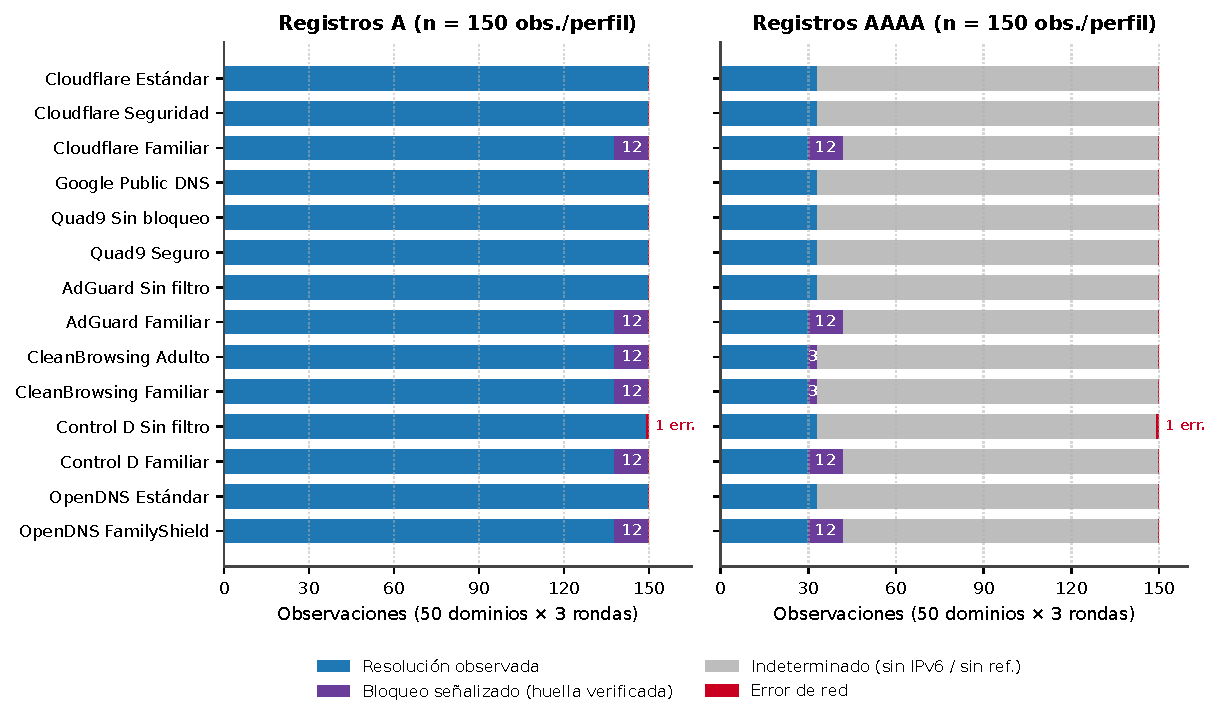
\includegraphics[width=\linewidth]{figuras/fig4_tcp_reclasificado.pdf}
\caption{Estados reclasificados con huellas verificadas por operador en los 14 perfiles TCP/53 sobre los 50 dominios base (150 observaciones por barra en A y AAAA; 2 errores de red totales en Control D Sin filtro).}
\label{fig:tcp-reclasificado}
\end{figure}

La figura \ref{fig:cobertura-pares} muestra la distribución de dominios consistentes comparables entre los 91 pares de perfiles TCP/53 tras la reclasificación. En \texttt{A}, 78 pares (85,7~\%) alcanzaron cobertura completa de 50/50 dominios y los 13 emparejados con Control D Sin filtro alcanzaron 49/50. En \texttt{AAAA}, la falta de publicación IPv6 en 39 de los 50 dominios (78,0~\%) redujo la cobertura a 11 dominios en 85 pares (93,4~\%), mientras 6 pares (entre los cuatro perfiles que inyectan respuestas sintéticas \texttt{AAAA} en los 3 sitios adultos sin IPv6) alcanzaron 14 dominios. Al cruzar los 15 pares posibles entre los seis perfiles parentales sobre estos 50 dominios documentales en \texttt{A}, todos produjeron acuerdo de 1,00 ($\kappa = 1{,}00$, $J = 1{,}00$, con 46 resoluciones y 4 bloqueos idénticos). Estos resultados validan el instrumento (objetivos 1 y 3) y confirman empíricamente la advertencia de Liu et al. \cite{liu2024} y OONI \cite{ooni2012}: sin calibrar páginas de bloqueo y sin separar el \texttt{NODATA} por falta de IPv6 de las fallas de red, las métricas se distorsionan. Al mismo tiempo, la saturación en 1,00 sobre 50 sitios conocidos demostró que se requiere un conjunto más amplio y diverso para diferenciar proveedores, ejecutado en la subsección \ref{subsec:doh}.

\begin{figure}[H]
\centering
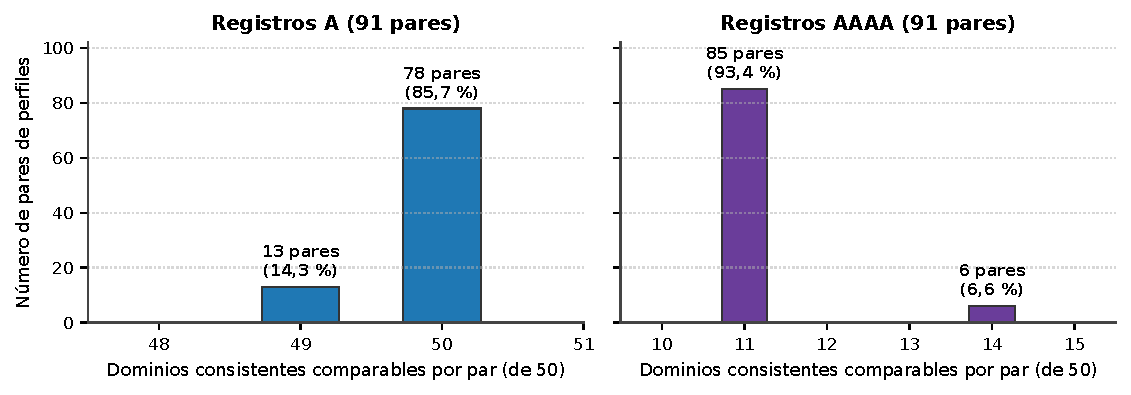
\includegraphics[width=0.92\linewidth]{figuras/fig5_cobertura_pares_reclasificado.pdf}
\caption{Distribución de dominios consistentes comparables entre los 91 pares de perfiles TCP/53 tras reclasificación con huellas verificadas, en registros A y AAAA.}
\label{fig:cobertura-pares}
\end{figure}

\subsection{Evaluación unificada de los 9 proveedores PDNS (20 perfiles DoH) y discrepancias}\label{subsec:doh}

Validado el esquema de huellas por operador, el 26 de noviembre de 2026 se ejecutó la campaña unificada por DoH HTTP/2 con verificación TLS sobre los \textbf{20 perfiles lógicos de los nueve proveedores DNS} frente al conjunto ampliado de \textbf{548 nombres} (543 dominios de evaluación con muestreo uniforme A--Z en los candidatos comunitarios, más 5 controles técnicos, 2 rondas, \texttt{A} y \texttt{AAAA}), sumando \textbf{43.840 consultas}. Durante esta ventana, los servidores cifrados de Mullvad continuaron respondiendo normalmente con certificados TLS válidos pese al retiro anunciado. En toda la campaña ocurrieron únicamente \textbf{4 errores de transporte} (0,009~\%, \textbf{99,99~\% de recepción}), todos en DNS4EU y con 0 errores en los otros 17 perfiles. Como detalla la tabla \ref{tab:consistencia} para cada uno de los 20 perfiles, la consistencia entre rondas sobre las consultas completadas fue de 99,6~\% a 100,0~\% en \texttt{A} y de 99,8~\% a 100,0~\% en \texttt{AAAA} (las escasas variaciones del 0,2~\% al 0,4~\% correspondieron a 1 o 2 dominios con fluctuación puntual de resolución entre rondas), con intervalos efectivos entre inicios de ronda de 35,5 s a 174,7 s (mediana de 80,9 s, reflejando la concurrencia secuencial acotada en DNS4EU, Control D y CleanBrowsing). En la referencia común (\texttt{1.1.1.1}), 499 de los 543 dominios estuvieron activos en \texttt{A} (42/42 apuestas Subtel, 22/22 adulto regulatorio, 13/13 armas, 166/166 educativo, 129/150 candidatos adultos de UT1 A--Z y 127/150 candidatos de apuestas de StevenBlack A--Z); los 21/150 dominios restantes de UT1 y 23/150 de StevenBlack resultaron inactivos en referencia (\emph{Indeterminado}) y quedaron fuera de los denominadores activos, reflejando la obsolescencia propia de listas comunitarias. En \texttt{AAAA}, 268 de los 543 dominios (49,4~\%) carecieron de registro IPv6 y solo 275 publicaron IPv6 (1/22 adulto regulatorio, 3/13 armas, 42/166 educativo, 23/42 Subtel, 120/150 candidatos adultos y 86/150 candidatos de apuestas).

\begin{table}[H]
\centering\scriptsize
\caption{Desempeño operativo individual de los 20 perfiles lógicos (2.192 consultas por perfil): errores de transporte (Err.), intervalo entre inicios de ronda ($\Delta t$), consistencia ante consultas repetidas (Cons.) y falsos positivos educativos en registro A (FP Edu. A) en la evaluación DoH de 43.840 consultas. *Los perfiles de CleanBrowsing emplean Cloudflare Estándar como referencia externa abierta.}
\label{tab:consistencia}
\begin{tabularx}{\textwidth}{Yrrrrr}
\toprule
Perfil DoH & Err. & $\Delta t$ (s) & Cons. A & Cons. AAAA & FP Edu. A\\
\midrule
Cloudflare Estándar (referencia abierta) & 0 & 41,4 & 100,0~\% & 100,0~\% & 0 / 166\\
Cloudflare Seguridad (amenazas) & 0 & 41,5 & 100,0~\% & 100,0~\% & 0 / 166\\
Cloudflare Familiar (parental) & 0 & 46,3 & 100,0~\% & 99,8~\% & 0 / 166\\
Google Public DNS (referencia externa) & 0 & 48,1 & 99,8~\% & 100,0~\% & 0 / 166\\
Quad9 Sin bloqueo (referencia abierta) & 0 & 56,3 & 100,0~\% & 100,0~\% & 0 / 166\\
Quad9 Seguro (amenazas) & 0 & 54,1 & 100,0~\% & 100,0~\% & 0 / 166\\
AdGuard Sin filtro (referencia abierta) & 0 & 77,8 & 100,0~\% & 100,0~\% & 0 / 166\\
AdGuard Predeterminado (seguridad y anuncios) & 0 & 78,8 & 99,6~\% & 99,8~\% & 0 / 165\\
AdGuard Familiar (parental) & 0 & 83,0 & 99,8~\% & 100,0~\% & 0 / 165\\
CleanBrowsing Adulto* (parental) & 0 & 115,4 & 100,0~\% & 100,0~\% & 0 / 165\\
CleanBrowsing Familiar* (parental) & 0 & 61,7 & 100,0~\% & 100,0~\% & 0 / 165\\
Control D Sin filtro (referencia abierta) & 0 & 160,2 & 100,0~\% & 100,0~\% & 0 / 166\\
Control D Familiar (parental) & 0 & 35,5 & 100,0~\% & 100,0~\% & 0 / 166\\
Cisco OpenDNS Estándar (referencia abierta) & 0 & 107,8 & 99,8~\% & 99,8~\% & 0 / 165\\
Cisco OpenDNS FamilyShield (parental) & 0 & 91,3 & 99,8~\% & 99,8~\% & 0 / 165\\
Mullvad Sin filtro (referencia abierta) & 0 & 85,4 & 100,0~\% & 100,0~\% & 0 / 165\\
Mullvad Familiar (parental) & 0 & 83,6 & 100,0~\% & 99,8~\% & 0 / 165\\
DNS4EU Sin filtro (referencia abierta) & 2 & 171,9 & 100,0~\% & 100,0~\% & 0 / 166\\
DNS4EU Protector (seguridad) & 1 & 174,7 & 99,8~\% & 100,0~\% & 0 / 165\\
DNS4EU Infantil (parental) & 1 & 168,1 & 100,0~\% & 100,0~\% & 0 / 166\\
\bottomrule
\end{tabularx}
\end{table}

La figura \ref{fig:benchmark-9} compara nueve perfiles evaluados de ocho proveedores DNS (los ocho perfiles parentales y Quad9 Seguro como línea base de amenazas; Google Public DNS y las variantes sin filtro operan como referencia) a través de los seis grupos en registros \texttt{A}, poniendo de relieve cuatro patrones diferenciados por categoría.

\textbf{Consenso en plataformas regulatorias frente a dispersión estructural en UT1 (adulto).} Los ocho perfiles parentales coincidieron al 100~\% en las 22 plataformas adultas regulatorias de UE/Ofcom (22/22). En contraste, sobre los 129 candidatos activos muestreados uniformemente A--Z desde UT1 \texttt{adult/domains}, la proporción bloqueada se polarizó en dos extremos: DNS4EU Infantil bloqueó 129/129 (100,0~\%) y AdGuard Familiar 128/129 (99,2~\%), frente a OpenDNS FamilyShield (16/129, 12,4~\%), Cloudflare Familiar (12/129, 9,3~\%), CleanBrowsing Adulto y Familiar (9/129, 7,0~\%), Mullvad Familiar (5/129, 3,9~\%) y Control D Familiar (1/129, 0,8~\%). El examen estructural por dominio raíz aporta una clave explicativa: incluso bajo muestreo uniforme sobre 4.590.350 entradas, 116 de los 129 dominios activos de UT1 (89,9~\%) correspondieron a subdominios \texttt{blogspot.*} (junto con 7 \texttt{tumblr.com}, 1 \texttt{free.fr} y 5 dominios independientes). Este patrón resulta consistente con la hipótesis de que DNS4EU y AdGuard incorporan listas comunitarias fuertemente solapadas con UT1 (incluidos subdominios históricos de alojamiento gratuito), mientras los demás proveedores parecen aplicar bases más selectivas, sin que sea posible verificar sus tuberías internas por no estar publicadas. No obstante, las discrepancias persistieron incluso entre los 5 dominios independientes: solo \texttt{puss8.com} alcanzó bloqueo unánime (8/8), mientras \texttt{tnaflicks.com}, \texttt{asiancelebs.win}, \texttt{dirtyindianx.net} (5/8) y \texttt{chaude-fellation-petasse.kekette.com} (3/8) dividieron a los proveedores.

\textbf{Apuestas en línea (Subtel Chile y candidatos de StevenBlack A--Z).} Al condicionarse cada perfil a la resolución estable en su propia referencia intra-proveedor (que resolvió entre 127 y 128 candidatos de StevenBlack) y excluir anomalías o indeterminados, los denominadores evaluables oscilaron entre 126 y 128 por perfil (167 a 169 en apuestas combinadas). Entre los dos perfiles gratuitos que declaran filtrar apuestas, DNS4EU Infantil bloqueó 40/42 sitios de Subtel (95,2~\%) y 127/127 candidatos comparables de StevenBlack (100,0~\%; un dominio adicional, \texttt{rizk.com}, devolvió \texttt{0.0.0.0} con TTL de 1 s en vez de la dirección de aviso calibrada \texttt{51.15.69.11} mientras DNS4EU Sin filtro resolvió direcciones ordinarias, por lo que quedó consolidado como indeterminado según la tabla \ref{tab:estados}), mientras Mullvad Familiar bloqueó 39/42 de Subtel (92,9~\%) y 126/127 candidatos (99,2~\%). Entre los proveedores que no declaran apuestas en su plan gratuito, Cloudflare y OpenDNS permitieron 42/42 sitios Subtel y bloquearon 2/126 (con un \texttt{NXDOMAIN} anómalo en \texttt{www.e-loterie.ma}) y 3/126 candidatos respectivamente; Control D Familiar bloqueó 8/127 candidatos (6,3~\%) y 1/42 de Subtel (\texttt{tikitaka.com}); CleanBrowsing Adulto y Familiar bloquearon 1/42 de Subtel (\texttt{cl.novibet.com}) y 0/127 candidatos; y AdGuard Familiar bloqueó 2/42 de Subtel (\texttt{melbet.com} y \texttt{www.jackpotcitycasino.com}) y 0/127 candidatos. Como AdGuard Predeterminado bloqueó 0/42 sitios Subtel y 0/127 candidatos, esos dos bloqueos ocurrieron exclusivamente en la capa familiar de AdGuard. En DNS4EU, la capa intermedia Protector bloqueó 2/42 sitios Subtel (\texttt{1wins.cl} y \texttt{playglobal5.com}) y 21/128 candidatos de apuestas (16,4~\%) por reglas de seguridad previas al perfil infantil.

\textbf{Armas (13 fabricantes oficiales).} Únicamente DNS4EU Infantil bloqueó los 13 fabricantes verificados (13/13, 100,0~\%), en concordancia con su política publicada \cite{dns4eupolitica}. Todos los demás perfiles parentales y Quad9 Seguro los resolvieron ordinariamente (0/13), acorde con que sus planes gratuitos no declaran cobertura de armamento.

\textbf{Cero bloqueos indebidos entre portales educativos y coherencia en registros \texttt{AAAA}.} No se observaron bloqueos educativos en ninguno de los 20 perfiles sobre los portales evaluables de cada uno: 0/166 en 11 perfiles (Cloudflare, Google, Quad9, Control D, AdGuard Sin filtro y DNS4EU Sin filtro e Infantil) y 0/165 en los 9 perfiles restantes. Esa diferencia de un portal en nueve perfiles respondió a respuestas \texttt{SERVFAIL} puntuales en tres dominios (\texttt{www.virginiawestern.edu} en AdGuard Predeterminado/Familiar, CleanBrowsing y OpenDNS; \texttt{point.edu} en Mullvad; y \texttt{www.rowan.edu} en DNS4EU Protector), que quedaron excluidos de esos denominadores por falta de resolución estable. En los 275 dominios que publicaron registro \texttt{AAAA}, los ocho perfiles parentales reprodujeron el mismo patrón por categoría que en \texttt{A}: 1/1 en adulto regulatorio, 120/120 en DNS4EU y 119/120 en AdGuard frente a 1/120 a 10/120 en los demás sobre UT1, 21/23 (DNS4EU) y 20/23 (Mullvad) en Subtel, 86/86 y 85/86 en StevenBlack, 3/3 solo en DNS4EU en armas y cero bloqueos educativos (0/41 en DNS4EU Infantil y 0/42 en los otros siete perfiles).

\begin{figure}[H]
\centering
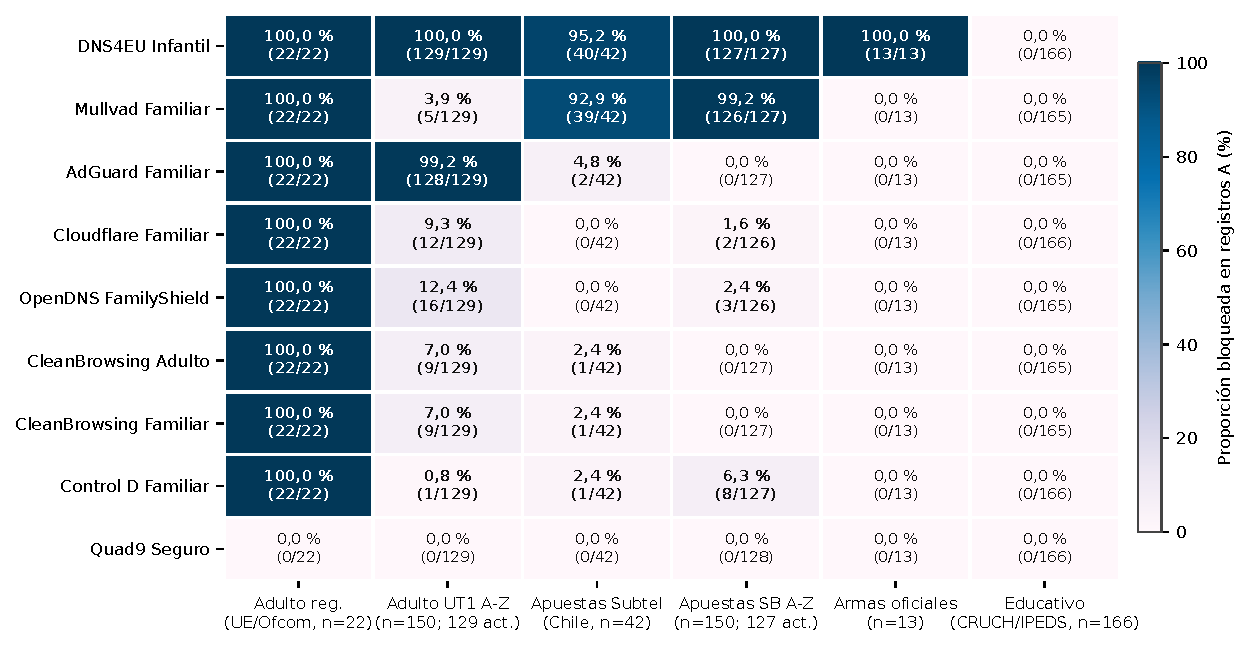
\includegraphics[width=\linewidth]{figuras/fig6_benchmark_9_proveedores.pdf}
\caption{Comparación unificada de proporción bloqueada en registros A para nueve perfiles evaluados de ocho proveedores DNS (los ocho perfiles parentales y Quad9 Seguro como línea base de amenazas; Google Public DNS y los perfiles sin filtro operan como referencia) sobre los seis grupos de 543 dominios (DoH HTTP/2, dos rondas; condicionado a resolución estable en la referencia intra-proveedor, o en Cloudflare Estándar como referencia externa abierta en CleanBrowsing, por lo que los activos en \texttt{1.1.1.1} indicados en el eje pueden variar en $\pm 1$ dominio por perfil).}
\label{fig:benchmark-9}
\end{figure}

Aplicando el criterio de exclusión de la subsección \ref{subsec:metodo-analisis}, las categorías de armas (bloqueada únicamente en 1/8 perfiles) y educativo (0/20 perfiles) quedaron fuera de las matrices pareadas por degeneración matemática. La figura \ref{fig:matrices-kj} muestra las matrices pareadas de Kappa de Cohen ($\kappa$, triángulo superior) y similitud de Jaccard ($J$, triángulo inferior) entre los ocho perfiles parentales en registros \texttt{A} para contenido adulto combinado ($n = 151$) y apuestas combinadas ($n = 167\text{--}169$). En \textbf{contenido adulto combinado ($n = 151$)}, DNS4EU Infantil y AdGuard Familiar alcanzaron una superposición casi total ($J = 0{,}99$, 150 bloqueos compartidos, con $\kappa = 0{,}00$ por efecto techo al bloquear DNS4EU 151/151). Frente a filtros de menor cobertura en listas comunitarias, el índice cayó hasta $J = 0{,}15$ (Control D frente a DNS4EU y AdGuard, con 23/151 bloqueos compartidos), $J = 0{,}18$ (Mullvad frente a ambos) y $J = 0{,}21$ (CleanBrowsing frente a ambos). Al aislar únicamente los \textbf{129 candidatos comunitarios de UT1} (sin las 22 plataformas regulatorias donde todos coincidieron), la divergencia se acentuó todavía más: frente a $J = 0{,}99$ entre AdGuard y DNS4EU, el índice cayó a $J = 0{,}008$ (1/129 frente a DNS4EU y 1/128 frente a AdGuard) para Control D, $J = 0{,}04$ (5/129 y 5/128) para Mullvad y $J = 0{,}07$ (9/129 y 9/128) para CleanBrowsing. Entre los perfiles con menor coincidencia con UT1 se observaron acuerdos altos sobre el conjunto combinado ($\kappa = 0{,}90$ y $J = 0{,}85$ entre Control D y Mullvad; $\kappa = 0{,}83$ y $J = 0{,}77$ entre CleanBrowsing y OpenDNS; $\kappa = 0{,}82$ y $J = 0{,}74$ entre CleanBrowsing y Control D). En \textbf{apuestas ($n = 167\text{--}169$)}, Mullvad Familiar y DNS4EU Infantil alcanzaron un acuerdo muy alto ($\kappa = 0{,}66$, $J = 0{,}99$, 164 bloqueos compartidos: 39/42 en Subtel con $\kappa = 0{,}79, J = 0{,}98$ y 125/126 en StevenBlack con $J = 0{,}99$). Los pares entre un perfil declarante de apuestas y uno no declarante alcanzaron como máximo $J = 0{,}054$ (Control D frente a DNS4EU); fuera de los declarantes destacaron CleanBrowsing Adulto frente a Familiar ($\kappa = 1{,}00$, $J = 1{,}00$, coincidiendo en \texttt{cl.novibet.com}) y Control D frente a OpenDNS ($\kappa = 0{,}49$, $J = 0{,}33$ por tres bloqueos compartidos en candidatos).

\begin{figure}[H]
\centering
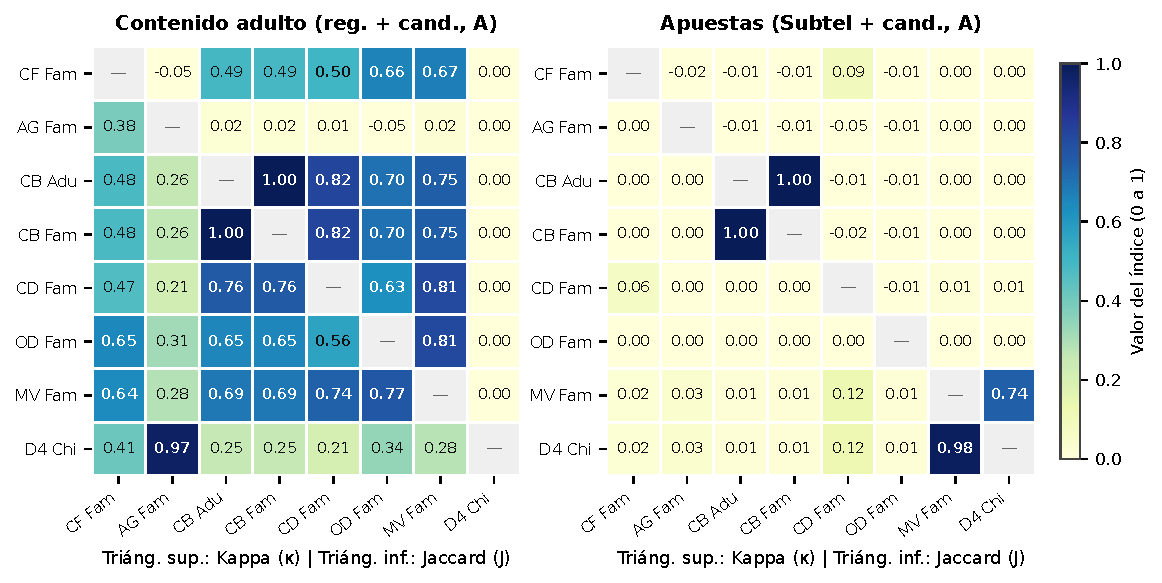
\includegraphics[width=\linewidth]{figuras/fig7_matrices_kappa_jaccard.pdf}
\caption{Matrices pareadas de coeficiente Kappa de Cohen ($\kappa$, triángulo superior) y similitud de Jaccard ($J$, triángulo inferior) entre los ocho perfiles parentales en registros A, separadas por contenido adulto combinado (izquierda, 151 dominios activos: 22 regulatorios y 129 candidatos UT1 A--Z) y apuestas combinadas (derecha, 167 a 169 dominios activos: 42 Subtel y candidatos StevenBlack A--Z). Abreviaturas de perfiles: \texttt{CF Fam} (Cloudflare Familiar), \texttt{AG Fam} (AdGuard Familiar), \texttt{CB Adu} y \texttt{CB Fam} (CleanBrowsing Adulto y Familiar), \texttt{CD Fam} (Control D Familiar), \texttt{OD Fam} (Cisco OpenDNS FamilyShield), \texttt{MV Fam} (Mullvad Familiar) y \texttt{D4 Inf} (DNS4EU Infantil).}
\label{fig:matrices-kj}
\end{figure}

En total se registraron \textbf{128 dominios concretos de discrepancia activa en candidatos adultos de UT1 A--Z}, \textbf{1 discrepancia directa en la nómina chilena de Subtel} (\texttt{estelarbet.cl}: bloqueado por DNS4EU Infantil y permitido por Mullvad Familiar), \textbf{2 omisiones compartidas por ambos filtros de apuestas en la nómina Subtel} (\texttt{latamwinonline.com} y \texttt{www.nayafacil-903.com}) y \textbf{1 discrepancia entre declarantes en candidatos de apuestas} (\texttt{rik.vip}: bloqueado por DNS4EU Infantil y permitido por Mullvad Familiar). La tabla \ref{tab:discrepancias} reúne ejemplos nominales verificados de estas discrepancias y omisiones, y la tabla \ref{tab:formatos-respuesta} resume los seis mecanismos distintos de reescritura DNS observados entre los ocho perfiles parentales.

\begin{table}[H]
\centering\scriptsize
\caption{Ejemplos nominales verificados de discrepancias y omisiones compartidas entre perfiles PDNS que declaran filtrar la categoría respectiva (registros A, medición del 26 de noviembre de 2026). Abreviaturas: Fam. (Familiar), Adu. (Adulto), Inf. (Infantil), FS (FamilyShield).}
\label{tab:discrepancias}
\begin{tabularx}{\textwidth}{>{\raggedright\arraybackslash}p{4.05cm}>{\raggedright\arraybackslash}p{2.20cm}>{\raggedright\arraybackslash}p{4.15cm}Y}
\toprule
Dominio observado & Grupo & Perfiles declarantes que bloquean (A) & Perfiles declarantes que permiten (A)\\
\midrule
\texttt{estelarbet.cl} & Apuestas Subtel & DNS4EU Inf. & Mullvad Fam.\\
\texttt{latamwinonline.com} & Apuestas Subtel & Ninguno (omisión compartida) & DNS4EU Inf., Mullvad Fam.\\
\texttt{www.nayafacil-903.com} & Apuestas Subtel & Ninguno (omisión compartida) & DNS4EU Inf., Mullvad Fam.\\
\texttt{rik.vip} & Apuestas SB A--Z & DNS4EU Inf. & Mullvad Fam.\\
\texttt{tnaflicks.com} & Adulto UT1 A--Z & AdGuard Fam., CleanBrowsing (Adu./Fam.), OpenDNS FS, DNS4EU Inf. & Cloudflare Fam., Control D Fam., Mullvad Fam.\\
\texttt{asiancelebs.win} & Adulto UT1 A--Z & Cloudflare Fam., AdGuard Fam., CleanBrowsing (Adu./Fam.), DNS4EU Inf. & Control D Fam., OpenDNS FS, Mullvad Fam.\\
\texttt{dirtyindianx.net} & Adulto UT1 A--Z & Cloudflare Fam., AdGuard Fam., OpenDNS FS, Mullvad Fam., DNS4EU Inf. & CleanBrowsing (Adu./Fam.), Control D Fam.\\
\texttt{beautifulgenitalia.tumblr.com} & Adulto UT1 A--Z & Cloudflare Fam., AdGuard Fam., CleanBrowsing (Adu./Fam.), OpenDNS FS, DNS4EU Inf. & Control D Fam., Mullvad Fam.\\
\bottomrule
\end{tabularx}
\end{table}

\begin{table}[H]
\centering\scriptsize
\caption{Seis mecanismos distintos de reescritura DNS observados entre los ocho perfiles parentales evaluados.}
\label{tab:formatos-respuesta}
\begin{tabularx}{\textwidth}{>{\raggedright\arraybackslash}p{3.05cm}>{\raggedright\arraybackslash}p{3.55cm}>{\raggedright\arraybackslash}p{4.05cm}Y}
\toprule
Perfil parental & Respuesta de bloqueo (A) & Respuesta de bloqueo (AAAA) & Mecanismo de reescritura\\
\midrule
Cloudflare Familiar & \texttt{0.0.0.0} + EDE 17 & \texttt{::} + EDE 17 & Sumidero + EDE explícito\\
AdGuard Familiar & \texttt{94.140.14.35} (sin EDE) & \texttt{NOERROR} + EDE 17 & Página de bloqueo (A) / EDE (AAAA)\\
CleanBrowsing (Adu./Fam.) & \texttt{NXDOMAIN} (sin EDE) & \texttt{NXDOMAIN} (sin EDE) & Respuesta negativa sintética\\
Control D Familiar & \texttt{0.0.0.0} (sin EDE) & \texttt{::} (sin EDE) & Sumidero sin EDE\\
OpenDNS FamilyShield & \texttt{146.112.61.106} (sin EDE) & \texttt{::ffff:146.112.61.106} (sin EDE) & Página de bloqueo IPv4 / mapeo IPv6\\
Mullvad Familiar & \texttt{NXDOMAIN} (sin EDE) & \texttt{NXDOMAIN} (sin EDE) & Respuesta negativa sintética\\
DNS4EU Infantil & \texttt{51.15.69.11} (\texttt{warning.joindns4.eu}, sin EDE) & \texttt{2001:bc8:1640:3ffd:}\newline\texttt{dc00:ff:fe4a:3ec9} (sin EDE) & Redirección a servidor de aviso\\
\bottomrule
\end{tabularx}
\end{table}

La tabla \ref{tab:formatos-respuesta} muestra además dos rasgos técnicos relevantes para el objetivo 1: solo dos de los ocho perfiles parentales emiten códigos EDE 17 (Cloudflare Familiar en ambos registros y AdGuard Familiar de forma asimétrica, devolviendo \texttt{94.140.14.35} sin EDE en \texttt{A} y \texttt{NOERROR} con EDE 17 en \texttt{AAAA}), mientras DNS4EU Infantil redirige tanto en IPv4 (\texttt{51.15.69.11}) como en IPv6 (\texttt{2001:bc8:1640:3ffd:dc00:ff:fe4a:3ec9}) al servidor \texttt{warning.joindns4.eu} documentado por Szymutko \cite{szymutko2026}. En perspectiva comparada con la literatura (objetivo 5), estos hallazgos extienden la taxonomía de reescritura de Liu et al. \cite{liu2024} al ámbito parental, corroboran la advertencia de Plonka et al. \cite{plonka2025} sobre el peso de subdominios históricos y entradas inactivas en listas abiertas, y matizan las brechas reportadas en Chile por Rojas et al. \cite{rojas2025,rojas2025ieee}: mientras la cobertura efectiva en sitios menos notorios, apuestas chilenas y armas varía drásticamente entre operadores, al aislar la capa DNS sobre portales universitarios institucionales verificados no se observaron falsos positivos educativos.

\subsection{Paridad entre cuatro transportes DNS: UDP/53, TCP/53, DoH y DoT/853}\label{subsec:transportes}

Dado que la campaña principal se ejecutó sobre DoH HTTP/2, el paso siguiente fue comprobar si el transporte DNS altera la política de filtrado aplicada por cada operador. En la madrugada del 26 de noviembre de 2026 (01:02--01:05 hora local de Chile, UTC-3) se ejecutó la prueba pareada de cuatro transportes sobre los 24 dominios documentados extraídos del conjunto de evaluación (2 rondas consecutivas sin reintentos), usando el mismo límite de espera de 2,5 s en UDP/53 y TCP/53 y de 3,5 s en DoH y DoT/853. Esto resolvió la ambigüedad de la observación inicial de octubre y permitió verificar el soporte efectivo de PDNS sobre DoT/853. La figura \ref{fig:transportes-4} resume la disponibilidad, la mediana del RTT y la paridad entre transportes.

Respecto de UDP/53, se observó una pérdida selectiva de respuestas desde la red residencial ensayada. Con idéntica espera de 2,5 s sobre el subconjunto pareado de 12 dominios en registro \texttt{A} (24 consultas por perfil), UDP/53 respondió normalmente hacia los tres resolutores públicos más conocidos: Cloudflare Estándar (\texttt{1.1.1.1}: 24/24, mediana 5,7 ms), Quad9 Seguro (\texttt{9.9.9.9}: 24/24, 5,5 ms) y Google Public DNS (\texttt{8.8.8.8}: 24/24, 56,8 ms). En cambio, agotó el tiempo en el \textbf{100~\% de las consultas (0/24)} hacia las siete direcciones restantes evaluadas en puerto 53 (incluidas \texttt{1.1.1.3} de Cloudflare Familiar y \texttt{9.9.9.10} de Quad9 Sin bloqueo, además de AdGuard, CleanBrowsing, Control D y OpenDNS). Sin embargo, \textbf{TCP/53 obtuvo 96/96 respuestas (100~\%) en los 10 perfiles de puerto 53} (medianas de 8,5 a 108,3 ms) con cero banderas \texttt{TC} de truncamiento. Esta diferencia a igual umbral de espera evidencia una pérdida o interferencia selectiva sobre el puerto 53/UDP en la ruta de acceso local, respaldada por la recuperación de respuestas UDP dentro del túnel de AdGuard VPN (subsección \ref{subsec:vpn-ooni}), y fundamenta el uso de TCP/53, DoH y DoT/853 en las campañas comparativas.

Sobre DoT en el puerto 853 (RFC 7858), se verificó que \textbf{los nueve operadores ofrecen soporte operativo en los 12 perfiles evaluados} con 100~\% de disponibilidad (96/96 en cada uno, con medianas RTT desde 30,9 ms en Quad9 Seguro y 35,2 ms en Control D Familiar hasta 520,8 ms en Mullvad Familiar y 911,5 ms en DNS4EU Infantil). En el caso particular de Cisco OpenDNS FamilyShield, el nombre de servidor dedicado a DoH (\texttt{doh.familyshield.opendns.com}) rechazó la conexión en el puerto 853 (\texttt{ConnectionRefusedError}). Sin embargo, consultar directamente la IP \texttt{208.67.222.123} por puerto 853 indicando el nombre de servidor TLS (\emph{Server Name Indication}, SNI) \texttt{dns.opendns.com} respondió 96/96 consultas (mediana 238,8 ms), aplicando el bloqueo FamilyShield en las 12 consultas \texttt{A} de contenido adulto (6 dominios $\times$ 2 rondas) y resolviendo los 4 portales educativos.

Al comparar par a par el estado de clasificación en cada tupla (\emph{perfil, dominio, tipo de registro, ronda}) donde ambos transportes respondieron, la paridad fue exactamente del \textbf{100,0~\% sin ninguna discrepancia}: 960/960 en TCP/53 frente a DoH, 960/960 en TCP/53 frente a DoT/853 y 1.152/1.152 en DoH frente a DoT/853, además de 72/72 en UDP/53 frente a TCP/53 sobre los tres perfiles alcanzables por UDP en esa red. Conviene precisar el alcance exacto de esta última cifra: como los tres perfiles que respondieron por UDP/53 (Cloudflare Estándar, Google Public DNS y Quad9 Seguro) no aplican filtrado parental y los siete perfiles restantes agotaron el tiempo en UDP/53, la conservación del filtrado parental queda acreditada entre \textbf{TCP/53, DoH y DoT/853}, mientras que en UDP/53 directo no pudo verificarse desde la red residencial ensayada (y sí se observó dentro del túnel de AdGuard VPN en la subsección \ref{subsec:vpn-ooni}).

\begin{figure}[H]
\centering
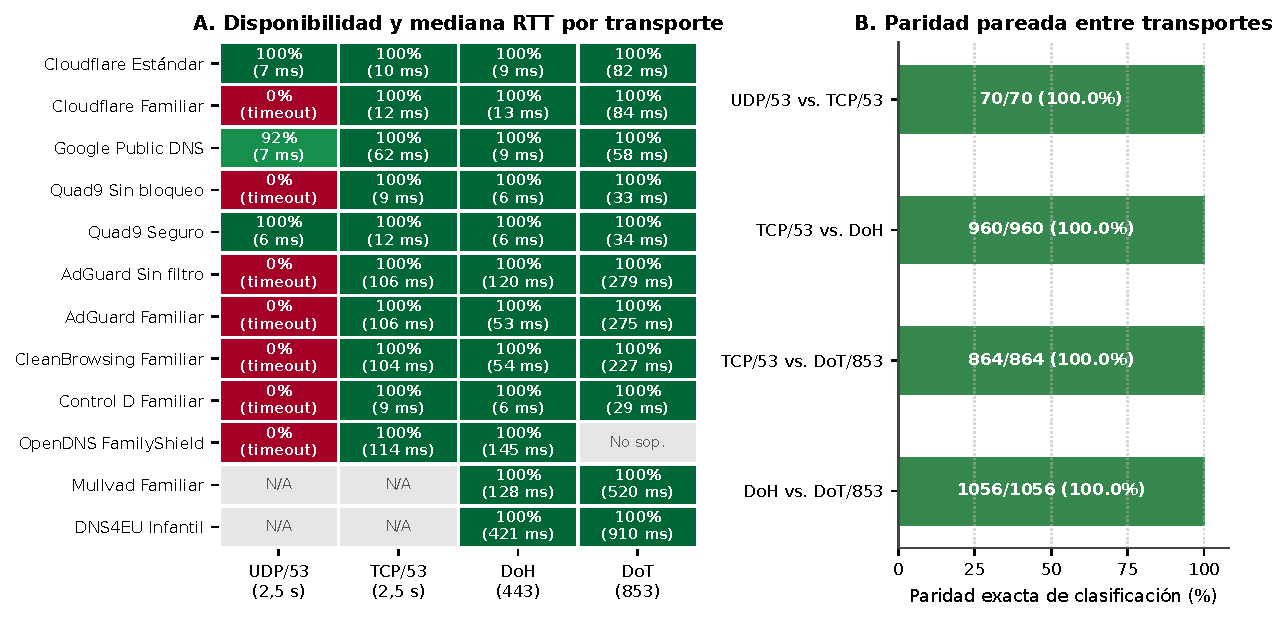
\includegraphics[width=\linewidth]{figuras/fig8_transportes_4_capas.pdf}
\caption{Disponibilidad, mediana del tiempo de ida y vuelta RTT (panel A) y paridad exacta de clasificación (panel B) en el ensayo pareado de cuatro transportes DNS (UDP/53 sobre 12 dominios en registro A a 2,5 s, con respuesta únicamente en tres perfiles sin filtro parental; TCP/53 a 2,5 s y DoH/DoT a 3,5 s sobre 24 dominios en A y AAAA; \texttt{N/A} indica que Mullvad y DNS4EU no operan resolutores públicos en puerto 53).}
\label{fig:transportes-4}
\end{figure}

\subsection{Evaluación bajo VPN, proxies y contraste externo con OONI en Chile}\label{subsec:vpn-ooni}

Comprobado el comportamiento de los resolutores directos en los cuatro transportes, resta evaluar qué ocurre cuando las consultas atraviesan túneles VPN o proxies y cómo se compara ese filtrado con registros públicos en redes chilenas. Para aislar el origen del filtrado cuando intervienen intermediarios, se combinaron controles causales de laboratorio con pruebas en cuatro servicios externos y la consulta al archivo público de OONI en Chile.

En el laboratorio aislado sobre dominios sintéticos \texttt{.test}, OpenVPN verificó el tránsito por \texttt{tun0}: el enlace directo y el túnel con la regla desactivada resolvieron las 24 observaciones por condición, mientras activar la regla en el resolutor del túnel produjo 18 señales de bloqueo sobre las tres categorías restringidas y 6 resoluciones en el control educativo. En el proxy HTTP local (12 solicitudes por condición), el acceso directo y el proxy sin regla devolvieron 12 respuestas exitosas \texttt{HTTP 200}, mientras activar la regla generó 9 respuestas \texttt{HTTP 403} (acceso prohibido) con huella documentada sobre las categorías restringidas y 3 respuestas \texttt{HTTP 200} en el grupo educativo (figura \ref{fig:vpn-proxy-lab}).

\begin{figure}[H]
\centering
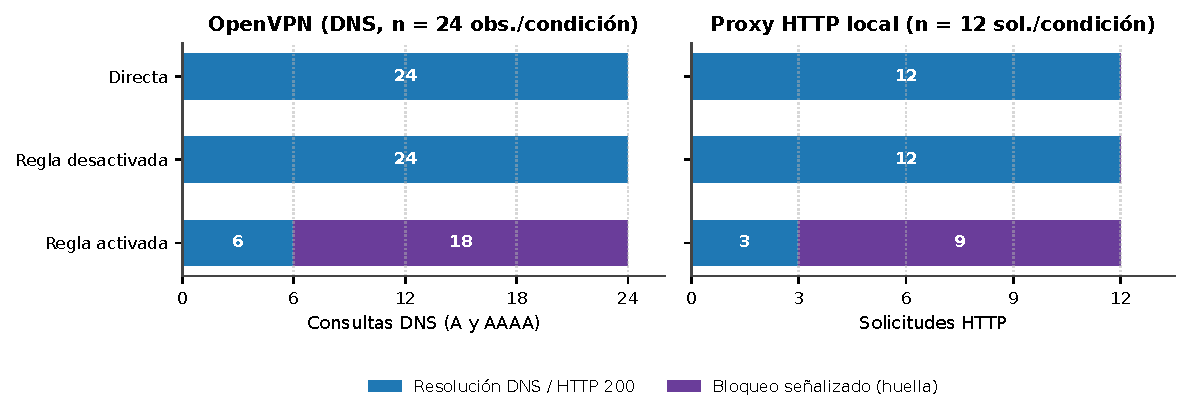
\includegraphics[width=\linewidth]{figuras/fig9_vpn_proxy_laboratorio.pdf}
\caption{Controles causales en laboratorio con OpenVPN (consultas DNS, 24 por condición) y proxy HTTP local (solicitudes HTTP, 12 por condición) bajo acceso directo, regla desactivada y regla activada.}
\label{fig:vpn-proxy-lab}
\end{figure}

En los servicios externos, la figura \ref{fig:vpn-externos} integra las mediciones DNS en los túneles de los tres operadores VPN (con una desviación de tamaño muestral entre sesiones: 15 dominios de contenido en la sesión inicial de WARP y 21 en las sesiones ampliadas de AdGuard VPN y RiseupVPN, lo que acota las comparaciones directas entre túneles a los grupos comunes), mientras que la tabla \ref{tab:proxies-externos} resume las solicitudes HTTPS \texttt{HEAD} a través de los tres proxies SOCKS5 externos (\texttt{socks5h}). El comportamiento verificado en cada intermediario se desglosa por servicio.

\textbf{Cloudflare WARP (\texttt{2026.8.2115.0}, plan gratuito).} Se ejecutó en un espacio de red aislado (\texttt{tap0} vía \texttt{slirp4netns 1.3.7}) con transporte cifrado MASQUE (sobre HTTP/3) y salida de enrutamiento distribuido \emph{anycast} verificada por diagnóstico HTTPS. Se registraron 228 respuestas DNS sobre 15 dominios de contenido (4 adultos, 4 apuestas, 3 armas y 4 educativos) más 4 controles técnicos (2 tipos de registro, 2 rondas) bajo ruta directa (\texttt{warp=off}), túnel sin filtro (\texttt{CloudflareWARP}) y túnel con filtro familiar (\texttt{family.cloudflare-dns.com}). Al activar el filtro familiar, los 4 dominios adultos pasaron de 8/8 direcciones ordinarias en \texttt{A} (y 2/8 en \texttt{AAAA}) a 8/8 sumideros \texttt{0.0.0.0}/\texttt{::} en ambos registros (junto con los controles de adulto y \emph{malware}), mientras apuestas, armas y educativo mantuvieron direcciones ordinarias en \texttt{A}. En modo proxy SOCKS5 (puerto \texttt{40000}, 32 solicitudes HTTPS \texttt{HEAD} en 2 rutas y 2 ajustes), aun con el filtro familiar activo, los controles de adulto y \emph{malware} devolvieron HTTP 200 por el proxy; cuatro solicitudes \texttt{GET} adicionales confirmaron cuerpos idénticos de 652 bytes con igual SHA-256 entre ruta directa y proxy, mientras \texttt{.invalid} falló antes de HTTP (\texttt{curl 6} directo y \texttt{curl 97} por proxy).

\textbf{AdGuard VPN para Linux (\texttt{v1.7.12}, plan gratuito).} Se probó en un contenedor descartable con salida fija verificada en Dallas (EE.~UU.), comparando 200 consultas directas de referencia por DoH desde Chile con 200 consultas UDP dentro del túnel (\texttt{tun0}, resolutor asignado \texttt{46.243.231.30}) sobre 25 nombres (4 adultos, 10 apuestas, 3 armas, 4 educativos y 4 controles). Dentro del túnel respondieron 199 de 200 consultas (un único tiempo agotado en un dominio de armas sin filtro), lo que respalda que la pérdida selectiva de UDP/53 observada en la subsección \ref{subsec:transportes} ocurre en la red de acceso local. Con DNS familiar activado en el túnel, los 4 dominios adultos devolvieron \texttt{94.140.14.35} en \texttt{A} (8/8) y EDE 17 en \texttt{AAAA} (8/8), frente a 8/8 direcciones ordinarias sin filtro; apuestas, armas y educativo resolvieron en \texttt{A}. En modo proxy SOCKS5 (puerto local \texttt{19080}, \texttt{socks5h}, salida verificada en Dallas), las 16 solicitudes HTTPS \texttt{HEAD} devolvieron HTTP 200 en los 3 controles válidos y \texttt{curl 6}/\texttt{curl 97} en \texttt{.invalid}. Como \texttt{nudity.testcategory.com} y \texttt{malware.testcategory.com} son controles propietarios de Cloudflare que AdGuard DNS no bloquea ni en modo túnel, esas solicitudes verifican conectividad HTTPS y resolución remota \texttt{socks5h}, mientras la no aplicación del DNS del túnel en modo SOCKS5 consta en el manual oficial del cliente \cite{adguardvpnlinux}.

\textbf{RiseupVPN (\texttt{OpenVPN 2.7.9}, servicio gratuito).} Con interfaz \texttt{tun0}, cifrado autenticado \texttt{AES-256-GCM}, salida verificada en París (\texttt{vpn02-par.riseup.net}) y resolutor interno \texttt{10.42.0.1} (\texttt{filter\_dns=false}), se ejecutaron 520 consultas DNS sobre 26 nombres (17 restringidos: 4 adultos, 10 apuestas [6 de Subtel y 4 del conjunto base] y 3 armas; 4 educativos y 5 controles) en cinco configuraciones: los dos perfiles DoH de DNS4EU (\texttt{Sin filtro} e \texttt{Infantil}) por ruta directa y por el túnel, más el resolutor UDP interno de Riseup. El estado coincidió exactamente en los 84 pares por perfil sobre los 21 dominios de contenido (21 dominios $\times$ 2 tipos $\times$ 2 rondas): los 17 dominios restringidos recibieron la dirección de aviso de DNS4EU en ambas rutas (34 consultas en \texttt{A}), mientras el resolutor interno de Riseup y el perfil abierto devolvieron direcciones ordinarias y los 4 portales educativos resolvieron sin bloqueo en las cinco configuraciones.

\textbf{Tor (\texttt{0.4.9.17} SOCKS5).} Como referencia externa de proxy sin política parental declarada (puerto local \texttt{19050}, salida verificada mediante el servicio de diagnóstico de Tor), se ejecutaron 16 solicitudes HTTPS \texttt{HEAD} sobre los 4 controles técnicos en dos rondas: los 3 nombres válidos devolvieron HTTP 200 tanto por ruta directa como por \texttt{socks5h}, mientras \texttt{.invalid} produjo \texttt{curl 6} en ruta directa y \texttt{curl 97} a través del proxy (tabla \ref{tab:proxies-externos}).

En conjunto, estos resultados confirman en el ámbito parental las observaciones de Khan et al. \cite{khan2018vpn} sobre la heterogeneidad del manejo DNS en clientes VPN (donde el mismo cliente WARP aplica el filtro familiar en modo túnel pero no en modo proxy SOCKS5) y validan la utilidad del contraste por integridad de cuerpo SHA-256 adaptado de Tsirantonakis et al. \cite{tsirantonakis2018proxy} para verificar que un proxy no modifica ni bloquea las respuestas HTTPS (objetivo 4).

\begin{figure}[H]
\centering
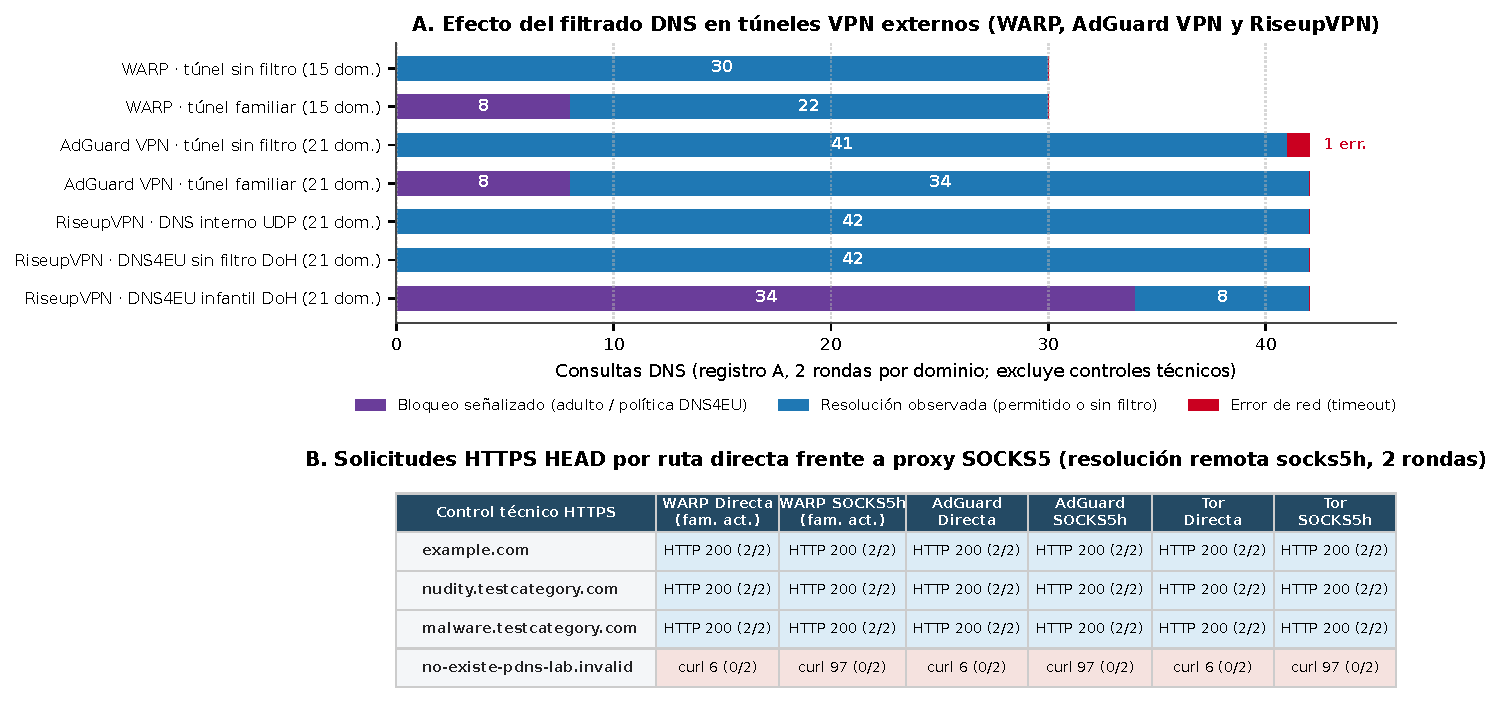
\includegraphics[width=\linewidth]{figuras/fig10_vpn_proxies_externos.pdf}
\caption{Efecto del filtrado DNS en registro A dentro de los túneles VPN externos de Cloudflare WARP (15 dominios de contenido), AdGuard VPN (21 dominios) y RiseupVPN (21 dominios), medidos en dos rondas por dominio excluyendo controles técnicos.}
\label{fig:vpn-externos}
\end{figure}

\begin{table}[H]
\centering\scriptsize
\setlength{\tabcolsep}{3.8pt}
\caption{Solicitudes HTTPS HEAD por ruta directa (dir.) frente a proxy SOCKS5 con resolución remota (\texttt{socks5h}, dos rondas por condición) en WARP (con filtro familiar activado), AdGuard VPN y Tor. \texttt{curl 6}: error de resolución DNS local; \texttt{curl 97}: error de conexión o resolución en el proxy SOCKS5.}
\label{tab:proxies-externos}
\begin{tabular}{lcccccc}
\toprule
Control técnico HTTPS & WARP dir. & WARP \texttt{socks5h} & AdGuard VPN dir. & AdGuard VPN \texttt{socks5h} & Tor dir. & Tor \texttt{socks5h}\\
\midrule
\texttt{example.com} & 200 (2/2) & 200 (2/2) & 200 (2/2) & 200 (2/2) & 200 (2/2) & 200 (2/2)\\
\texttt{nudity.testcategory.com} & 200 (2/2) & 200 (2/2) & 200 (2/2) & 200 (2/2) & 200 (2/2) & 200 (2/2)\\
\texttt{malware.testcategory.com} & 200 (2/2) & 200 (2/2) & 200 (2/2) & 200 (2/2) & 200 (2/2) & 200 (2/2)\\
\texttt{no-existe-pdns-lab.invalid} & \texttt{curl 6} (2/2) & \texttt{curl 97} (2/2) & \texttt{curl 6} (2/2) & \texttt{curl 97} (2/2) & \texttt{curl 6} (2/2) & \texttt{curl 97} (2/2)\\
\bottomrule
\end{tabular}
\end{table}

Para contrastar estos resultados con el acceso registrado en redes locales chilenas, se consultó el archivo público de OONI Explorer para Chile (\texttt{probe\_cc=CL}, septiembre a noviembre de 2026), que registró 277.556 mediciones \emph{Web Connectivity} en el país (5.579 anomalías y 1 bloqueo confirmado). Al consultar los 84 dominios documentados del estudio mediante las cuatro variantes de URL con un tope de 50 mediciones más recientes por URL (\texttt{limit=50}), solo 4 dominios arrojaron historial en esa ventana, sumando \textbf{194 mediciones recientes en siete ASN chilenos} (\texttt{AS7418}, \texttt{AS14117}, \texttt{AS22047}, \texttt{AS27651}, \texttt{AS27901}, \texttt{AS264827} y \texttt{AS272105}). Los otros 80 dominios (41 de Subtel, 1 de UE DSA [\texttt{stripchat.com}], 18 de Ofcom, 13 de armas, 6 universitarios y \texttt{example.com}) no registraron mediciones públicas en Chile en esa ventana (tabla \ref{tab:ooni-chile}). La figura \ref{fig:ooni-chile} compara la tasa de anomalías reportadas en los cuatro dominios con historial: el sitio de apuestas de Subtel \texttt{juegalo.com} acumuló \textbf{37 anomalías en 44 mediciones (84,1~\%)} tras la instrucción de septiembre de 2026, mientras las tres plataformas adultas (\texttt{pornhub.com}, \texttt{xnxx.com} y \texttt{xvideos.com}, cada una en el tope de 50 registros) sumaron solo \textbf{4 anomalías en 150 mediciones}, es decir, \textbf{146 de 150 mediciones sin anomalía reportada (97,3~\%)} en los mismos siete ASN. Conforme a la guía de interpretación de OONI \cite{ooni}, estos registros agregados reflejan mediciones voluntarias sin documentar la configuración DNS local de cada sonda ni desagregar todos los posibles fallos de red; aun bajo ese límite, el contraste sugiere que en los ASN chilenos observados las tres plataformas adultas permanecieron mayoritariamente accesibles sin intervención del ISP.

\begin{table}[H]
\centering\scriptsize
\setlength{\tabcolsep}{3.6pt}
\caption{Cobertura por categoría de los 84 dominios consultados en OONI Explorer para Chile (siete ASN, septiembre--noviembre de 2026). *Consulta acotada a un máximo de 50 mediciones más recientes por URL (\texttt{limit=50}); las tres plataformas adultas alcanzaron dicho tope.}
\label{tab:ooni-chile}
\begin{tabular}{lrrrrr}
\toprule
Categoría consultada en OONI (CL) & Consultados & Con registros & Sin registros & Mediciones* & Anomalías\\
\midrule
Apuestas (Subtel) & 42 & 1 (\texttt{juegalo.com}) & 41 & 44 & 37 (84,1~\%)\\
Adulto (UE DSA) & 4 & 3 (\texttt{pornhub.com}, \texttt{xnxx.com}, \texttt{xvideos.com}) & 1 & 150 & 4 (2,7~\%)\\
Adulto (Ofcom) & 18 & 0 & 18 & 0 & 0\\
Armas (fabricantes oficiales) & 13 & 0 & 13 & 0 & 0\\
Educativo (muestra universitaria) & 6 & 0 & 6 & 0 & 0\\
Control técnico (\texttt{example.com}) & 1 & 0 & 1 & 0 & 0\\
\midrule
Total & 84 & 4 & 80 & 194 & 41\\
\bottomrule
\end{tabular}
\end{table}

\begin{figure}[H]
\centering
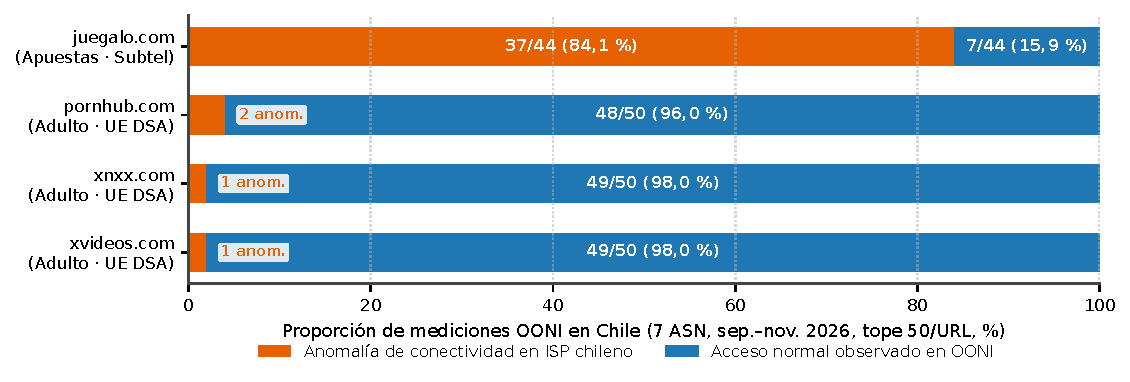
\includegraphics[width=0.92\linewidth]{figuras/fig11_ooni_chile.pdf}
\caption{Proporción de mediciones con y sin anomalía reportada en OONI Explorer sobre siete ASN chilenos (septiembre--noviembre de 2026, tope de 50 mediciones por URL) para el sitio de apuestas de Subtel (\texttt{juegalo.com}) y tres plataformas adultas globales.}
\label{fig:ooni-chile}
\end{figure}

\Needspace{6\baselineskip}
\section{Conclusiones}

En respuesta a la pregunta de investigación, los nueve servicios públicos gratuitos de \emph{Protective DNS} (PDNS) evaluados (20 perfiles lógicos) exhiben una consistencia a corto plazo elevada ante consultas repetidas sobre transportes orientados a conexión (99,6~\% a 100,0~\% en \texttt{A} y 99,8~\% a 100,0~\% en \texttt{AAAA} en 43.840 consultas DoH, con 100~\% de paridad de filtrado parental entre TCP/53, DoH y DoT/853). Sin embargo, divergen sustancialmente tanto en sus formatos de reescritura DNS como en su cobertura efectiva fuera de los sitios más notorios y en categorías como apuestas y armas. Distinguir señales de filtrado respecto de fallas de red o respuestas negativas legítimas exige combinar perfiles de referencia medidos en la misma ventana (intra-proveedor en ocho operadores y Cloudflare Estándar como referencia externa en CleanBrowsing), controles técnicos conocidos (\texttt{.invalid} y servidores de aviso calibrados dinámicamente) y un esquema de clasificación calibrado por operador que incorpore EDE 15--17, descarte EDE 18 como prueba suficiente de bloqueo y separe explícitamente el \texttt{NODATA} por falta de IPv6 y los fallos \texttt{SERVFAIL} de los errores de transporte.

El objetivo general se cumplió en sus dimensiones centrales, con un grado de cumplimiento diferenciado entre los seis objetivos específicos. Los \textbf{objetivos 1, 3 y 6 se cumplieron íntegramente}: se caracterizaron seis mecanismos distintos de reescritura DNS entre los ocho perfiles parentales (confirmando la adopción minoritaria de EDE 17, presente solo en Cloudflare Familiar y AdGuard Familiar en \texttt{AAAA}, y verificando el servidor de aviso \texttt{warning.joindns4.eu} documentado por Szymutko \cite{szymutko2026}), se demostró mediante reclasificación TCP/53 que omitir estas huellas o el 49,4~\% a 80,0~\% de ausencia IPv6 distorsiona las métricas (extendiendo la taxonomía de Liu et al. \cite{liu2024} al ámbito parental), y quedaron documentados y públicos el paquete \texttt{pdns-lab} (30 pruebas unitarias y SQLite), los scripts multitransporte/OONI y los registros reproducibles.

Los \textbf{objetivos 2, 4 y 5 se cumplieron en el núcleo experimental con limitaciones acotadas y transparentes}. En el \textbf{objetivo 2}, la auditoría retiró 94 entradas sintácticamente inválidas, excluyó 266 dominios de incitación al odio (UT1 \texttt{agressif}) mal rotulados como armas y detectó el truncamiento alfabético de las listas heredadas (100~\% prefijo \texttt{0} en adultos y 95,8~\% en \texttt{0--9}/\texttt{a} en apuestas), consolidando un conjunto auditable de 548 nombres con muestreo uniforme A--Z y 166 portales universitarios verificados por HTTPS (corroborando empíricamente la advertencia de Plonka et al. \cite{plonka2025}); no obstante, el inventario heredado de 2.000 candidatos conserva 934 entradas sin revisión manual individual (400 Tranco y 534 \texttt{liste\_bu}) junto con 33 portales educativos no verificados en portada. En el \textbf{objetivo 4}, los controles de laboratorio (OpenVPN y proxy HTTP local, cuya regla activa produjo 9/9 bloqueos HTTP 403 en categorías restringidas y 3/3 respuestas HTTP 200 en el control educativo) y los tres túneles VPN externos (WARP, AdGuard VPN y RiseupVPN) confirmaron que el bloqueo depende del resolutor DNS o de la regla activa y no del túnel por sí mismo (coincidiendo con el manejo heterogéneo de DNS en VPN reportado por Khan et al. \cite{khan2018vpn} y validando el contraste de integridad SHA-256 adaptado de Tsirantonakis et al. \cite{tsirantonakis2018proxy}); su cumplimiento es parcial respecto de los tres proxies SOCKS5 externos, que carecen de política parental propia y se evaluaron únicamente sobre controles técnicos HTTPS.

En el \textbf{objetivo 5}, escalar de 50 dominios base a 543 dominios reveló brechas ocultas en la muestra inicial y refina en la capa DNS los resultados chilenos de Rojas et al. \cite{rojas2025,rojas2025ieee}: los ocho filtros parentales coincidieron en 22/22 plataformas adultas regulatorias, pero sobre los 129 candidatos activos A--Z de UT1 (donde 89,9~\% correspondió a subdominios \texttt{blogspot.*}) el bloqueo osciló entre 0,8~\% (Control D) y 12,4~\% (OpenDNS) frente a 99,2~\% (AdGuard) y 100,0~\% (DNS4EU), reduciendo la similitud de Jaccard a $J = 0{,}15$ sobre los 151 dominios adultos combinados y a $J = 0{,}008$ al aislar los 129 candidatos comunitarios, con discrepancias persistentes incluso en dominios independientes (\texttt{tnaflicks.com}, \texttt{asiancelebs.win}, \texttt{dirtyindianx.net}). En apuestas, solo DNS4EU Infantil (40/42 Subtel; 127/127 StevenBlack) y Mullvad Familiar (39/42 Subtel; 126/127 StevenBlack) ofrecieron cobertura amplia ($\kappa = 0{,}66$, $J = 0{,}99$), con dos omisiones compartidas en Subtel (\texttt{latamwinonline.com} y \texttt{www.nayafacil-903.com}) y discrepancias en \texttt{estelarbet.cl} (Subtel) y \texttt{rik.vip} (StevenBlack), ambos bloqueados por DNS4EU Infantil y permitidos por Mullvad Familiar (los dos únicos perfiles declarantes de apuestas). En armas, solo DNS4EU Infantil bloqueó los 13 fabricantes oficiales (13/13 frente a 0/13). A diferencia de los falsos positivos descritos en aplicaciones móviles de control parental \cite{rojas2025ieee}, no se observaron bloqueos educativos en ninguno de los 20 perfiles (0/165 a 0/166 en \texttt{A}; 0/41 a 0/42 en \texttt{AAAA}). Asimismo, la paridad de filtrado parental alcanzó el 100,0~\% entre TCP/53, DoH y DoT/853 (960/960 TCP/DoH, 960/960 TCP/DoT y 1.152/1.152 DoH/DoT, verificando soporte DoT/853 en los nueve operadores), pero quedó acotada parcialmente en UDP/53 directo porque la pérdida selectiva en la red local solo permitió contrastar 72/72 observaciones en los tres perfiles sin filtro parental (observándose filtrado UDP dentro del túnel de AdGuard VPN). El contraste con OONI \cite{ooni2012,ooni} sobre 194 mediciones en siete ASN chilenos mostró 37/44 anomalías reportadas (84,1~\%) en \texttt{juegalo.com} frente a 146/150 mediciones sin anomalía reportada (97,3~\%) en tres plataformas adultas, quedando 80/84 dominios sin historial público en la ventana consultada.

Las principales contribuciones del estudio comprenden un marco reproducible de auditoría y medición DNS/VPN/proxy, un conjunto de evaluación trazable que evidencia la vulnerabilidad de las listas comunitarias frente a sesgos léxicos y subdominios de alojamiento gratuito, y evidencia empírica directa sobre la oferta gratuita disponible en Chile. Para familias, establecimientos educativos e investigadores, estos resultados implican que elegir un perfil PDNS gratuito por su nombre comercial no garantiza cobertura en apuestas o armamento ni homogeneidad en sitios adultos fuera de las plataformas más populares, y que activar una VPN con filtro familiar no asegura protección al utilizar su modo proxy SOCKS5. Finalmente, la validez de estas conclusiones permanece sujeta a seis condiciones materiales: la observación desde una única red residencial en Chile (con interferencia local sobre UDP/53), una ventana temporal acotada entre octubre y noviembre de 2026 con intervalos entre rondas dentro de los TTL habituales (consistencia a corto plazo frente a listas dinámicas no publicadas), el carácter intencional y no probabilístico del corpus, el retiro anunciado de los servidores públicos cifrados de Mullvad, la restricción a planes gratuitos y capa DNS (sin verificar accesibilidad HTTP/HTTPS/SNI en sitios restringidos ni extensiones de navegador) y la naturaleza voluntaria y acotada (\texttt{limit=50}, sin registro del DNS local) de las sondas de OONI Explorer.

\section{Trabajo futuro}\label{sec:futuro}

En coherencia con las limitaciones y cumplimientos parciales declarados en las conclusiones, los trabajos posteriores se dividen en aspectos pendientes del alcance original y nuevas líneas de investigación proyectadas hacia memoria o tesis de título.

\textbf{Aspectos pendientes o acotados del alcance original:}
\begin{enumerate}
\item \textbf{Revisión manual individual del inventario de 2.000 candidatos:} completar la verificación individual con evidencia, responsable y fecha de las 934 entradas no categorizadas (Tranco y \texttt{liste\_bu}), los 33 portales educativos sin portada verificada y los candidatos comunitarios del conjunto de evaluación.
\item \textbf{Verificación directa de paridad parental en UDP/53:} repetir el ensayo pareado de cuatro transportes desde redes sin interferencia selectiva sobre el puerto 53/UDP para acreditar la paridad parental en UDP/53 directo frente a TCP/53, DoH y DoT/853.
\item \textbf{Proxies externos con política parental propia y pruebas sobre dominios reales:} evaluar proxies externos que declaren filtrado de contenido y extender las pruebas SOCKS5 desde los cuatro controles técnicos hacia dominios parentales reales en un conjunto común entre clientes VPN.
\end{enumerate}

\textbf{Nuevas líneas de investigación proyectadas:}
\begin{enumerate}[resume]
\item \textbf{Seguimiento longitudinal y dinámica de bases de categorización:} aprovechar la herramienta y los registros reproducibles para medir la evolución temporal de las listas que alimentan a los proveedores de PDNS (incluido el retardo desde la aparición o sanción regulatoria de un dominio hasta su bloqueo efectivo, y si persisten las omisiones en \texttt{latamwinonline.com}, \texttt{www.nayafacil-903.com} y \texttt{estelarbet.cl}).
\item \textbf{Contraste multi-ISP en Chile, DNS sobre QUIC y corridas propias de OONI Probe:} medir el cumplimiento de la orden de Subtel (42 sitios de apuestas), el acceso a contenido adulto y el soporte de DNS sobre QUIC (\emph{Quick UDP Internet Connections}, DoQ) en múltiples ISP residenciales chilenos (Movistar, Entel, VTR, Claro y Mundo), complementado con ejecuciones propias del cliente activo \emph{OONI Probe} para cubrir los 80 dominios sin historial público en OONI Explorer.
\item \textbf{Planes comerciales de pago y ámbito de navegador:} contrastar los perfiles gratuitos frente a planes configurables de pago (CleanBrowsing configurable, Windscribe R.O.B.E.R.T. y el DNS interno en túnel WireGuard de Mullvad tras el retiro de sus servidores públicos), así como comparar extensiones de navegador frente a clientes de sistema y ampliar las pruebas de falsos positivos hacia sitios educativos temáticamente sensibles (educación sexual y salud).
\item \textbf{Verificación de accesibilidad en capa de aplicación (HTTP/HTTPS y SNI):} complementar la medición DNS con pruebas controladas de conectividad TCP/TLS y campo SNI para detectar bloqueos fuera de DNS (inspección de SNI, bloqueo por IP o páginas inyectadas) y evaluar la eficacia de extremo a extremo.
\item \textbf{Índice compuesto de confiabilidad y respuestas DNS explicables:} proponer un índice compuesto que pondere cobertura por categoría, consistencia temporal, ausencia de falsos positivos educativos y transparencia de señalización (EDE), así como diseñar respuestas de bloqueo DNS explicables apoyadas en campos estándar como \texttt{EXTRA-TEXT} de EDE (RFC 8914) para informar categoría y criterio aplicado.
\end{enumerate}

\Needspace{7\baselineskip}
\begingroup
\footnotesize
\setlength{\parskip}{0pt}
\phantomsection
\addcontentsline{toc}{section}{Referencias}
\bibliographystyle{IEEEtran}
\bibliography{referencias}
\endgroup
\end{document}
